% numerical.tex

\cleardoublepage
\chapter{Optimised Trajectory Including Fly-Back}\label{chapter:Flyback}
\textcolor{red}{ XXX Its interesting if the SPARTAN is flying close to its min q at first hump}
	
This chapter presents the maximum payload-to-orbit trajectory of the rocket-scramjet-rocket launch system, with the fly-back of the scramjet accelerator included within the optimal trajectory calculation performed by LODESTAR. 
Flying back the scramjet accelerator for landing at the initial launch site is one of the primary enabling factors in the cost efficient operation of the launch system. If the scramjet accelerator is launched onto a trajectory from which it is not able to fly-back, it must perform a downrange landing, likely at an Indonesian airfield when launched northerly from north Australia. This would necessitate transporting the scramjet accelerator back to Australia, a costly and time consuming process, and would require for international landing facilities to be available. 
Flying back the scramjet accelerator during the launch process removes the need for costly transportation from a downrange launch site, and allows for rapid refurbishment and re-use.
In addition, if a launch site is used from which there is no downrange landing site, the scramjet accelerator must necessarily fly-back to the initial launch site. 


\begin{figure}[ht]% updated 15/8/19
	\centering
	\includegraphics[width=1\linewidth]{H:/github-home/LODESTAR-revisions/ArchivedResults/20190723T110354mode11/GroundTrackStandard}
	\caption{Maximum payload-to-orbit trajectory path with the inclusion of scramjet accelerator fly-back (Case 11). Initial heading angle of \textcolor{red}{3.3}$^\circ$.} % note the heading angle at 10s is used
	\label{fig:GroundTrackStandard}
\end{figure}

The fly-back of the scramjet accelerator requires turning-around the scramjet accelerator after third stage separation, covering the necessary ground distance for return, and decelerating to reduce the speed of the scramjet accelerator to landing approach velocity, while maintaining a suitable descent angle to allow for a controlled approach. 
The return of the scramjet accelerator to the initial launch site is included in the optimisation process to assess whether it is possible for the fly-back of the scramjet accelerator to be achieved as a part of the launch process, and to maximise the overall payload-to-orbit efficiency of the launch system. This is compared to the optimised, maximum payload-to-orbit trajectory without fly-back (detailed in Chapter \ref{chapter:Ascent}) to assess the detrimental effects of the fly-back on the performance of the launch system. 
A sensitivity analysis is conducted, in a similar fashion to Chapter \ref{chapter:Ascent}. 
This sensitivity analysis allows the influence of the fly-back of the scramjet accelerator on the design sensitivities of the launch system to be analysed.


\section{Case 11: SPARTAN Trajectory with Scramjet Accelerator Return}
\begin{table}[ht] % upodated 14/8/19
	\centering
\begin{tabular}{l c } 
	\hline \textbf{Trajectory Condition}
	&Value 
	\\
	\hline \textbf{Payload to Orbit (kg)}
	& \textbf{\PayloadToOrbitStandard}
	\\
	\textbf{Total $\eta_{exergy}$ (\%)}
	& \textbf{\totalExergyEffStandard}
	\\
	\hline 
	\textbf{1$^{st}$ Stage $\eta_{exergy}$ (\%)}
	& \textbf{\firstExergyEffStandard}
	\\

	\textbf{Separation Alt, 1$\rightarrow$2 (km)}
	& \firstsecondSeparationAltStandard
	\\
	\textbf{Separation v, 1$\rightarrow$2 (m/s)}
	& \firstsecondSeparationvStandard
	\\
	\textbf{Separation $\gamma$, 1$\rightarrow$2 (deg)}
	& \firstsecondSeparationgammaStandard
	\\
	\hline 
	\textbf{2$^{nd}$ Stage $\eta_{exergy}$ (\%)}
	& \textbf{\secondExergyEffStandard}
	\\

	\textbf{Separation Alt, 2$\rightarrow$3 (km)}
	& \secondthirdSeparationAltStandard
	\\
	\textbf{Separation $v$, 2$\rightarrow$3 (m/s)}
	& \secondthirdSeparationvStandard
	\\
	\textbf{Separation $\gamma$, 2$\rightarrow$3 (deg)}
	& \secondthirdSeparationgammaStandard
	\\

	\textbf{2$^{nd}$ Stage Distance Flown (km)}
	& \SecondDistStandard
	\\
	\textbf{2$^{nd}$ Stage Return Fuel (kg)}
	& \returnFuelStandard
	\\
	\textbf{2$^{nd}$ Stage Return Distance (km)}
	& \returnDistStandard
	\\
	\hline 
	\textbf{3$^{rd}$ Stage $\eta_{exergy}$ (\%)}
	& \textbf{\thirddExergyEffStandard}
	\\

	\textbf{3$^{rd}$ Stage $t$, $q >$ 5kpa (s)}
	& \thirdqOverFiveStandard
	\\
	\textbf{3$^{rd}$ Stage Fuel Mass (kg)}
	& \thirdmFuelStandard
	\\
	\hline 
\end{tabular} 
\caption{Selected trajectory conditions for a maximum payload-to-orbit trajectory including scramjet accelerator fly-back (Case 11).}
\end{table}

LODESTAR is used to optimise the trajectory of the rocket-scramjet-rocket launch system, including the return of the scramjet accelerator to its initial launch site. The optimised trajectory is shown in Figure \ref{fig:GroundTrackStandard}. 
The rocket-scramjet-rocket launch system is shown to be able to successfully launch a small satellite to sun synchronous orbit, 
while flying-back the scramjet accelerator to the initial launch site location, and approaching the landing site at appropriately low altitude and velocity to allow for landing. 
The optimised trajectory attains a payload mass to SSO of \PayloadToOrbitStandard kg, a \textcolor{red}{-24.3}kg (\textcolor{red}{-15.5}\%) reduction in payload mass compared to the optimised ascent-only trajectory, detailed in Chapter \ref{chapter:Ascent}. 
The benefits of flying back the scramjet accelerator to its initial launch site, compared to the alternative of transporting the scramjet accelerator back to the launch site from a remote landing, are likely to far outweigh this associated reduction in payload. 



\section{Ascent Trajectory}

\begin{figure}[ht]% updated 14/8/19
	\centering
	\includegraphics[width=0.9\linewidth]{H:/github-home/LODESTAR-revisions/ArchivedResults/20190723T110354mode11/FirstStageStandard}
	\caption{The first stage of the optimised maximum payload-to-orbit trajectory with scramjet accelerator fly-back (Case 11). }
	\label{fig:FirstStageStandard}
\end{figure}
When the fly-back of the scramjet accelerator is included in the trajectory optimisation, the shape of the ascent trajectory of the launch system is altered significantly, compared to the ascent-only trajectory, detailed in Chapter \ref{chapter:Ascent}.
 The first stage initially pitches towards the east, beginning at a heading angle of \textcolor{red}{-12.45}$^\circ$.
 After pitchover, the first stage gradually reduces the angle of attack to a minimum of -0.47$^\circ$ at 30.9s flight time, in order to make small adjustments to the pitch profile while the velocity is low. After this, the first stage angle of attack returns to 0$^\circ$ at 42.9s flight time, and is maintained for 16.4s. \textcolor{red}{XXX update all this first stage stuff}
 The angle of attack is then reduced, to a minimum of -3.58$^\circ$ in order to adjust the altitude and trajectory angle, before increasing back to 0$^\circ$ at first-second stage separation. 
 The scramjet accelerator is released in an easterly direction, at a heading angle of \textcolor{red}{2.16}$^\circ$, an altitude of \firstsecondSeparationAltStandard km, and a trajectory angle of \firstsecondSeparationgammaStandard $^\circ$. 
 The altitude of first-second stage separation is 3.02km (+12.5\%) higher than the first-second stage separation point with no fly-back, with a trajectory angle at separation which is +2.5$^\circ$ (+80.6\%) higher. 
 This higher release point requires less aerodynamic manoeuvring of the first stage, and enables the first stage to be efficiently launched with a higher fuel mass of 17943kg, an increase of +758kg (+4.4\%) compared to the trajectory without fly-back. This additional fuel increases the total acceleration of the first stage, \textcolor{red}{XXX change all this too}
 in turn increasing the exergy efficiency of the first stage rocket by +0.308\%$\eta$ (+4.9\%) due to a higher propulsion efficiency, and allowing the first stage to achieve a higher velocity at separation (an increase of +64m/s, +4.3\%). 
 
  \begin{figure}[!ht] % updated 14/8/19
  	\centering
  	\includegraphics[width=1\linewidth]{H:/github-home/LODESTAR-revisions/ArchivedResults/20190723T110354mode11/SecondStageStandard}
  	\caption{The acceleration of the scramjet accelerator flying an optimised maximum payload-to-orbit trajectory with scramjet accelerator fly-back (Case 11). }
  	\label{fig:SecondStageStandard}
  \end{figure}
  \textcolor{red}{XXX change the first part of this}
 The higher altitude, larger trajectory angle, and increased velocity at the first-second stage separation point causes an altitude raising manoeuvre at the beginning of the scramjet accelerator's acceleration, which is significantly higher than the altitude raising manoeuvre with no fly-back. This altitude raising manoeuvre takes the scramjet accelerator to an altitude of \textcolor{red}{32.3}km at \textcolor{red}{47.1}s, and decreases the dynamic pressure of the scramjet accelerator to \textcolor{red}{14.9}kPa, allowing time for the bank angle of the scramjet accelerator to be increased. 
 After the first-second stage separation, the bank angle is increased, at the maximum change rate, to \textcolor{red}{52.2}$^\circ$, which aids the scramjet accelerator in decreasing its altitude. As the altitude of the scramjet accelerator begins to reduce, the bank angle \textcolor{red}{reduces} and the angle of attack is raised to \textcolor{red}{3.9}$^\circ$ to increase lift, slowing the descent of the scramjet accelerator. 
 The bank angle then begins to increase once more, and as the scramjet accelerator reaches close to its maximum dynamic pressure at \textcolor{red}{122.5}s, the bank angle reaches its maximum of \textcolor{red}{66.2}$^\circ$. 

After this point, the bank angle of the scramjet accelerator is maintained between \textcolor{red}{48.0}$^\circ$ and \textcolor{red}{52.5}$^\circ$, exhibiting higher bank angles towards the latter part of the ascent. At the end of the scramjet accelerator's ascent, the bank angle is reduced, so that the third stage is released at 0$^\circ$ bank angle. This 0$^\circ$ bank angle is defined as a constraint on the end of the trajectory, to ensure that the third stage rocket is released in the vertical plane, and is able to manoeuvre to orbit. 


The angle of attack of the scramjet accelerator is significantly higher over the course of the maximum payload-to-orbit trajectory with fly-back inclusion, compared to maximum payload-to-orbit trajectory with no fly-back, detailed in Section \ref{sec:optimisednoreturn}. These significantly  higher angles of attack are a result of the high bank angle of the scramjet accelerator throughout its trajectory, which cause the lift of the scramjet accelerator to be partially used for changing the heading of the scramjet accelerator, rather than providing vertical force. 
 The higher angles of attack result in the optimal trajectory of the scramjet accelerator following a close to maximum dynamic pressure path for most of the duration of its trajectory, without the altitude raising manoeuvre observed in Section \ref{sec:optimisednoreturn}.
 The increase in angle of attack means that the scramjet accelerator no longer flies within the homogeneous region of the specific impulse of the C-REST engines. instead the flight conditions are close to a region where an increase in angle of attack causes a sharp decrease in specific impulse, illustrated in Figure \ref{fig:NetIspStandard}. 
This indicates that the angle of attack, and consequently the allowable bank angle, of the scramjet accelerator is being limited by the performance of the C-REST engines. 
 The scramjet accelerator stays close to its maximum dynamic pressure until a pull-up is performed at \textcolor{red}{386.6}s flight time. 
 \begin{figure}[!ht]% updated 14/8/19
 	\centering
 	\includegraphics[width=\linewidth]{H:/github-home/LODESTAR-revisions/ArchivedResults/20190723T110354mode11/NetIspStandard}
 	\caption{Net $I_{SP}$ contours for the scramjet accelerator at Mach numbers between 5.5 and 8.5, showing the optimised trajectory path (Case 11). }
 	\label{fig:NetIspStandard}
 \end{figure}

The higher angles of attack flown by the scramjet accelerator also have the consequence of decreasing the net specific impulse of the scramjet accelerator during its acceleration, with the maximum specific impulse being decreased by -\textcolor{red}{3.4}\%.
The overall exergy efficiency of the scramjet accelerator is decreased, to \secondExergyEffStandard\%$\eta$, a decrease of \textcolor{red}{-0.643}\%$\eta$ (\textcolor{red}{-14.6}\%) compared to the maximum payload-to-orbit trajectory with no fly-back. This exergy efficiency decrease is due partially to the decrease in the specific impulse of the scramjet engines, but more significantly is attributed to the fuel necessary for the return flight resulting in less fuel being available for the ascent of the scramjet accelerator, and thus less `useful' work being attained from the total fuel mass.
A total fuel mass of \textcolor{red}{1304.2}kg is used during the scramjet accelerator's acceleration, out of a total of 1562kg of available fuel. This reduction in fuel mass used, along with the reduction in net specific impulse due to the higher angle of attack values, reduces the velocity at second-third stage separation by \textcolor{red}{-134.0}m/s (\textcolor{red}{-5.1}\%) compared to the maximum payload-to-orbit case with no scramjet accelerator fly-back. The scramjet accelerator pulls up to \secondthirdSeparationAltStandard km altitude and \secondthirdSeparationgammaStandard $^\circ$ trajectory angle before the second-third stage separation, a difference of only \textcolor{red}{-0.94}km (\textcolor{red}{-2.1}\%) and \textcolor{red}{+0.4}$^\circ$ (\textcolor{red}{+3.3}\%) compared to the maximum payload-to-orbit trajectory without fly-back, indicating that the inclusion of fly-back does not have a large effect on the magnitude of the pull-up manoeuvre. 

The exergy efficiency of the third stage is decreased by \textcolor{red}{-2.386}\%$\eta$ (\textcolor{red}{-15.4}\%) when compared to the maximum payload-to-orbit trajectory with no scramjet accelerator fly-back. This lowered efficiency is primarily due to the lower velocity of the third stage release, which increases the losses of the third stage due to propulsive inefficiencies. 


\begin{figure}[ht!]% updated 14/8/19
\centering
\includegraphics[width=1\linewidth]{H:/github-home/LODESTAR-revisions/ArchivedResults/20190723T110354mode11/ThirdStageStandard}
\caption{The third stage trajectory of an optimised maximum payload-to-orbit trajectory with scramjet accelerator fly-back (Case 11). }
\label{fig:ThirdStageStandard}
\end{figure}


\section{Fly-Back Trajectory}

\begin{figure}[ht!] % updated 14/8/19
	\centering
	\includegraphics[width=1\linewidth]{H:/github-home/LODESTAR-revisions/ArchivedResults/20190723T110354mode11/ReturnStandard}
	\caption{The fly-back trajectory of the scramjet accelerator flying an optimised maximum payload-to-orbit trajectory (Case 11). }
	\label{fig:ReturnStandard}
\end{figure}

The optimised fly-back trajectory is shown in Figure \ref{fig:ReturnStandard}.
The scramjet accelerator is shown to be capable of fly-back, using \returnFuelStandard kg of fuel, \textcolor{red}{16.5}\% of the total fuel.
Throughout its fly-back the scramjet accelerator performs distinct skipping manoeuvres, and ignites the scramjet engines a total of three times. 
These skips are consistent with previous research which has shown that a periodic skipping trajectory increases the downrange distance achievable by hypersonic vehicles both during powered and unpowered flight\cite{Moshman2014,Darby2011,Toso2015,Tetlow1992,Eggers1957,Kanda2007,Chai2015}, and serve to reduce the fuel necessary for the return flight. 

It is observed that the optimised trajectory exhibits characteristics which can be separated into three distinct segments; 1. initial turn, 2. boost-skip, and 3. approach, as indicated in Figure \ref{fig:ReturnStandard}. 
 
\subsubsection{ Initial Turn}
The scramjet accelerator separates from the third stage rocket at a bank angle of 0$^\circ$, and then increases its bank angle at close to the maximum change rate until \textcolor{red}{94.5}s return flight time, at which point \textcolor{red}{ the maximum of 90.0}$^\circ$ bank angle is reached. This high bank angle serves to rapidly change the heading of the scramjet accelerator, in order to minimise the down-range distance flown, and reduce the fuel necessary for fly-back. 
The angle of attack is kept low during this time, in order to minimise the size of the initial skip. 
As the scramjet accelerator reaches the zenith of its initial skip, at \textcolor{red}{73.6}s flight time and \textcolor{red}{66.5}km altitude, the angle of attack is rapidly increased, up to the maximum of \textcolor{red}{10.0}$^\circ$. 
This increase in angle of attack generates additional lift to slow the descent of the scramjet accelerator into the trough of the first skip, ensuring that the dynamic pressure limit is not exceeded. 


\subsubsection{ Boost-Skip}\label{sec:boost}
At \textcolor{red}{194.1}s flight time, the scramjet engines are ignited. The C-REST engines are powered-on in the trough between the first and second skips, at a point of high potential specific impulse, and initially burn for \textcolor{red}{33.8}s. During the initial burn, the L/D of the scramjet accelerator increases significantly, due to the scramjet engine flow paths of the scramjet accelerator generating thrust, rather than drag. 
This increase in L/D raises the altitude of the scramjet accelerator and, along with heavy banking, changes the heading of the scramjet accelerator significantly. 
The burn is limited by the lower inlet dynamic pressure limit of the C-REST engines, of 20kPa, and terminates at \textcolor{red}{227.9}s flight time. After the initial burn ends, the angle of attack of the scramjet accelerator is decreased to 3.2$^\circ$, and the scramjet accelerator executes its second skip. Once the scramjet accelerator is descending again, and as soon as the dynamic pressure is high enough for C-REST engine operation at \textcolor{red}{369.0}s return flight time, the scramjet engines are once again ignited.
During the second burn, the angle of attack of the scramjet accelerator is increased, to modify the temperature and Mach number at the inlet of the C-REST engines so that the maximum specific impulse is obtained from the C-REST engines during the burn. 
The angle of attack varies between \textcolor{red}{4.7}$^\circ$ to \textcolor{red}{3.7}$^\circ$ during the second burn, and the L/D is once again raised significantly, initiating the third skip. 
This skip raises the altitude of the scramjet accelerator to \textcolor{red}{53.3}km, before it decreases once again. 
The third and last burn is initiated at \textcolor{red}{581.7}s and lasts until \textcolor{red}{615.9}s, when the remaining fuel has been depleted. Before the third burn, the angle of attack is \textcolor{red}{first increased up to 7.5$^\circ$, and then decreased at the beginning of the burn, to a minimum of 4.1}$^\circ$ during the burn. The angle of attack values observed are similar to those observed during the second burn, indicating that these angle of attack values obtain a high specific impulse from the C-REST engines, this can be observed in Figure \ref{fig:returnIspStandard}, which shows the specific impulse profile of the return flight during the boost-skip phase. 

After the third burn phase, the angle of attack is initially controlled so that the skipping trajectory of the scramjet accelerator is dampened.
Immediately after the third burn phase, the angle of attack is reduced, to \textcolor{red}{2.84}$^\circ$. This reduction coincides with the ascent portion of the fourth skip, reducing the lift, and the amount of altitude gained. 
As the zenith of the forth skip is reached, the angle of attack is increased to \textcolor{red}{7.5}$^\circ$, increasing the lift, and once again slowing the descent. 
This high angle of attack is \textcolor{red}{increased until 984.9s, in stages corresponding with the descent of the last two small skips}.
It is notable that the \textcolor{red}{angle of attack is controlled in this way during the unpowered portion of the trajectory, as it indicates that the skips are being damped.} This implies that some degree of skipping is desirable after the final scramjet burn, but that the angle of attack is being controlled to produce optimally sized skips. 

\subsubsection{Approach}

After the final small skip, at \textcolor{red}{1046.0}s flight time, the angle of attack is adjusted, so that a gradual, controlled descent is initiated. 
After the skip phase, as the vehicle is approaching Mach 1, the angle of attack is reduced gradually to bring the scramjet accelerator down below 1km altitude, in a controlled manner. At \textcolor{red}{1455.0}s, the bank angle is increased, in order to perform a final adjustment of the heading angle, to bring the scramjet accelerator to the desired end location. 
The scramjet accelerator drops below 1km altitude at \textcolor{red}{-17.0}$^\circ$ trajectory angle and \textcolor{red}{95.2}m/s velocity (Mach 0.28). It is assumed that the scramjet accelerator is able to perform a landing manoeuvre after this point. 





\section{Energy Usage Analysis}


\begin{table}[!ht]% updated 29/12/19
	\centering
	\begin{tabular}{l c c} 
		\hline \textbf{Trajectory Condition}
		& No Fly-Back
		& With Fly-Back
		\\
		\textbf{First Stage Fuel Exergy} 
		&\textbf{\firstEnergyStandardNoReturn} GJ
		&\textbf{\firstEnergyStandard} GJ
		\\
		
		\textcolor{blue}{KE + PE of Payload}
		& \firstWpayloadStandardNoReturn \% (0.22 GJ)
		& \firstWpayloadStandard \% (0.19 GJ)
		\\
		\textcolor{red}{KE + PE of  2$^{nd}$ \& 3$^{rd}$ Stage}
		& \firstWnextStageStandardNoReturn \% (13.66 GJ)  & \firstWnextStageStandard \% (13.79 GJ)
		\\
		\textcolor{red}{Overcoming Drag} 
		& \WDoneStandardNoReturn \% (5.03 GJ) & \WDoneStandard \% (4.87 GJ)
		\\
		\textcolor{red}{KE + PE of 1$^{st}$ Stage Structural Mass} 
		& \WoneStandardNoReturn \% (2.04 GJ) & \WoneStandard \% (2.06 GJ)
		\\
		\textcolor{red}{KE + PE of 1$^{st}$ Stage Fuel Mass} 
		& \WmFoneStandardNoReturn \% (5.39 GJ) & \WmFoneStandard \% (5.41 GJ)
		\\ 
		\textcolor{red}{Propulsion Inefficiency} 
		& \PlossoneCombinedStandardNoReturn \% (180.95 GJ) & \PlossoneCombinedStandard \% (181.00 GJ)
		\\ 
		\textbf{Scramjet Accelerator Fuel Exergy} 
		& \textbf{\secondEnergyStandardNoReturn} GJ & \textbf{\secondEnergyStandard} GJ
		\\
		\textcolor{blue}{KE + PE of Payload}
		& \secondWpayloadStandardNoReturn \% (0.39 GJ) & \secondWpayloadStandard \% (0.28J)
		\\
		\textcolor{red}{KE + PE of 3$^{rd}$ Stage}
		& \secondWnextStageStandardNoReturn \% (7.85 GJ) & \secondWnextStageStandard \% (6.76 GJ)
		\\
		\textcolor{red}{Overcoming Drag}
		& \WDsecondStandardNoReturn \% (38.26 GJ) & \WDsecondStandard \% (33.56 GJ)
		\\
		\textcolor{red}{KE + PE of Scramjet Accelerator Structural Mass}  
		& \WsecondStandardNoReturn \% (12.39 GJ) & \WsecondStandard \% (10.58 GJ)
		\\
		\textcolor{red}{KE + PE of scramjet accelerator Fuel Mass}  
		& \WmFsecondStandardNoReturn \% (2.49 GJ) & \WmFsecondStandard \% (2.27 GJ)
		\\
		\textcolor{red}{Propulsion Inefficiency}  
		& \PlosssecondStandardNoReturn \% (126.01 GJ) & \PlosssecondStandard \% (103.00 GJ)
		\\
		
		
		
		\textbf{Return Fuel Exergy} 
		& - & \textbf{\returnEnergyStandard} GJ
		\\
		KE + PE of Scramjet Accelerator Structural Mass
		& - & \WreturnStandard \% (-17.61 GJ)
		\\
		\textcolor{red}{Overcoming Drag}
		& - & \WDreturnStandard \% (29.47 GJ)
		\\
		\textcolor{red}{KE + PE of scramjet accelerator Fuel Mass}  
		& - & \WmFreturnStandard \% (-0.51 GJ)
		\\
		\textcolor{red}{Propulsion Inefficiency}  
		& - & \PlossreturnCombinedStandard \% (19.56 GJ)
		\\
		
		
		\textbf{Third Stage Fuel Exergy}  
		& \textbf{\thirdEnergyStandardNoReturn} GJ & \textbf{\thirdEnergyStandard} GJ
		\\
		\textcolor{blue}{KE + PE of Payload}  
		&\thirddExergyEffAtmStandardNoReturn \% (0.73 GJ) &\thirddExergyEffAtmStandard \% (0.72 GJ)
		\\
		\textcolor{red}{Overcoming Drag}  
		& \WDthreeStandardNoReturn \% (0.11 GJ) & \WDthreeStandard \% (0.12 GJ)
		\\
		\textcolor{red}{KE + PE  of 3$^{rd}$ Stage Structural Mass}  
		& \WthreeStandardNoReturn \% (1.34 GJ) & \WthreeStandard \% (1.57 GJ)
		\\
		
		\textcolor{red}{KE + PE  of 3$^{rd}$ Stage Fuel Mass}  
		& \WmFthreeStandardNoReturn \% (9.28 GJ) & \WmFthreeStandard \% (10.30 GJ)
		\\
		
		\textcolor{red}{KE + PE of Heat Shield}  
		
		& \WHSthreeStandardNoReturn \% (1.22 GJ) & \WHSthreeStandard \% (1.41 GJ)
		\\
		
		\textcolor{red}{Propulsion Inefficiency}  
		& \PlossthreeStandardNoReturn \% (4.10 GJ) & \PlossthreeStandard \% (4.58 GJ)
		\\
		\textbf{Circularisation and Hohman Transfer Fuel Exergy}  
		& \textbf{\HTExergyStandardNoReturn}  GJ & \textbf{\HTExergyStandard}  GJ
		\\
		\textcolor{blue}{KE + PE of Payload}  
		& \HTeffStandardNoReturn \% (4.60 GJ) & \HTeffStandard \% (3.83 GJ)
		\\
		\textcolor{red}{All Other Energy Losses}  
		& \HTlossStandardNoReturn \% (14.46 GJ) & \HTlossStandard \% (13.62 GJ)
		\\
		\hline 
	
	\end{tabular} 
	\caption{An energy usage breakdown of the ascent trajectories, both with, and without, scramjet accelerator fly-back (Cases 11 \& 2). Blue indicates a 'productive' energy usage, whereas red indicates energy 'wastage'. Negative energy indicates energy being supplied.}
	\label{tab:effStandard}
\end{table}


An energy usage analysis is conducted for a maximum payload-to-orbit trajectory, including the fly-back of the scramjet accelerator. This is compared to the energy usage breakdown of the optimised trajectory without the fly-back of the scramjet accelerator in Table \ref{tab:effStandard}. Similarly to Section \ref{sec:exergy1}, the energy used to accelerate the payload is shown, along with the energy imparted to the successive stages; the energy used overcoming drag; the energy used imparting energy to the structural mass of each stage, which is separated; and the energy lost due to propulsion inefficiency. 



The fly-back of the scramjet accelerator reduces the fuel, and thus the fuel exergy, available to the scramjet accelerator during ascent.
This lower exergy, along with the altered manoeuvrability needs of the scramjet accelerator when the fly-back is included, results in a raising of the altitude and trajectory angle at the first-second stage separation. The increased altitude and trajectory angle at separation increases the fuel mass that the first stage rocket is able to use efficiently, and also increases the exergy efficiency of the first stage, partly compensating for the decrease in the efficiency of the scramjet accelerator due to fly-back. Overall, when the fly-back is included, more of the exergy of the first stage is utilised imparting energy upon the combination of the payload and the successive stages, at \textcolor{red}{6.92}\% (\textcolor{red}{13.97} GJ), compared to \textcolor{red}{6.87}\% (\textcolor{red}{13.87} GJ) without scramjet accelerator fly-back. This is due to the rocket flying a more efficient trajectory, with lower drag and propulsive losses, terminating at a higher altitude and velocity.



When flying a trajectory where the scramjet accelerator's fly-back is included, the drag losses during the ascent of the scramjet accelerator consist of a larger percentage of the ascent fuel exergy usage  (\WDsecondStandard \%, compared to \WDsecondStandardNoReturn \% without fly-back). This is despite the lower velocity range over which the scramjet accelerator is accelerating when fly-back is included, and is due to the less favourable first-second stage separation conditions, as well as the high banking throughout the acceleration. 
The energy necessary to return the scramjet accelerator to its initial launch location is provided by both the fuel used during the return (\textcolor{red}{30.92} GJ), as well as the kinetic and potential energy imparted upon the scramjet accelerator during its ascent (\textcolor{red}{12.85} GJ). Significantly more energy is required to overcome drag during the return (\textcolor{red}{29.47} GJ) than is available from the kinetic and potential energy of the scramjet accelerator (\textcolor{red}{17.61} GJ), illustrating the necessity for igniting the scramjet engines during the return flight. 


When the fly-back is included, the second-third stage separation occurs at a lower altitude and velocity, and the lower fuel exergy of the scramjet accelerator during its ascent results in less energy being imparted upon the payload and third stage by the scramjet accelerator (\textcolor{red}{7.04} GJ), compared to the trajectory without fly-back (\textcolor{red}{8.24} GJ). 
The lower, slower separation point when fly-back is included causes the losses of the third stage to increase from all sources, and for more energy to be used exiting the atmosphere. 


\section{Design Sensitivity Analysis}\label{sec:sensitivity}

\textcolor{red}{XXX make the argument that these parametetrs are for trjectory studues and to inform designers on criticality of coefficients}
\textcolor{red}{XXX remove max aoa}
It has been shown that the fly-back of the scramjet accelerator has a significant effect on the performance of the rocket-scramjet-rocket launch system, and that the maximum payload-to-orbit optimised trajectory changes significantly to compensate for the additional requirement of successfully returning the scramjet accelerator stage. This section investigates the sensitivity of the launch system to changes in the vehicle design, with the fly-back of the scramjet accelerator included. This sensitivity study varies the following:
\begin{itemize}
	\item Case 12: Dynamic Pressure, 
	\item Case 13: Specific Impulse,
	\item Case 14: Scramjet Accelerator Drag,
	\item Case 15: Scramjet Accelerator Mass,
	\item Case 16: Scramjet Accelerator Fuel Mass,
	\item Case 17: Third Stage Mass,
	\item Case 18: Third Stage Thrust.
\end{itemize}
As in Section \ref{sec:sensitivityNoReturn}, the effect of third stage drag is negligible. For this reason, variation in the third stage drag is omitted from this study. 

The launch system is able to successfully place a small satellite in orbit for every performance condition which has been tested, while returning the scramjet accelerator to its initial launch location for landing. 
Every maximum payload-to-orbit optimised trajectory exhibits considerable banking during the scramjet accelerator's ascent trajectory, as well as a pull-up of the scramjet accelerator before third stage release. 
In every case the optimised return flight path exhibits initial turn, boost-skip and approach phases. 
However, the height, and duration of the second skip of the return phase varies between cases, exhibiting no clear trend across the majority of the sensitivity studies which have been performed.

The first-second stage separation angle and altitude show no clear trend in any of the sensitivity studies performed, except for the third stage mass variation, in contrast to the sensitivity studies with no fly-back, detailed in Section \ref{sec:sensitivityNoReturn}, in which the scramjet accelerator mass and drag parameters change the first stage separation point significantly. All of the optimised trajectory solutions show a distinct initial altitude raising manoeuvre performed by the scramjet accelerator, however, the size is inconsistent across optimised trajectory solutions, indicating that this manoeuvre is no longer solely a product of an efficiency trade-off between the first stage pitching and scramjet accelerator engine efficiency.
In the maximum payload-to-orbit optimised trajectories calculated during the sensitivity analysis, it is observed that the trajectory angle at the first-second stage separation varies significantly between the optimised trajectories, with no discernible trend. When the scramjet accelerator is released at a high trajectory angle, the first stage is able to use more fuel, and fly a more efficient trajectory. In contrast to the trajectory with no fly-back,
releasing the scramjet accelerator at a higher trajectory angle and altitude causes it to spend a significant amount of time in a low dynamic pressure environment, giving time for the bank angle to increase. The high bank angle is utilised during the descent of the scramjet accelerator onto the maximum dynamic pressure path, to rapidly change the heading of the scramjet accelerator. This mitigates some of the reduction in efficiency caused by a higher first-second separation point.
 A lower release angle results in the first stage flying a slightly less efficient trajectory. However, a lower release angle also results in the scramjet accelerator using its fuel more rapidly, and manoeuvring more at the beginning of its trajectory, which results in the fly-back requiring less fuel. 
The trade-off between first stage efficiency and the initial operational efficiency of the scramjet accelerator appears to be close, and 
for each particular trajectory optimisation one or the other is favoured with no clear trend. 


It is also observed that there are two distinct return trajectory shapes for the return trajectory of the scramjet accelerator. The more common return trajectory shape has been shown in the preceding section, and consists of three or more large skips to begin the return trajectory. The second trajectory shape exhibits a small second skip, with the first two burns very closely spaced, or combined into one longer burn. An example of this second type of return trajectory is shown in Figure \ref{fig:ReturnComparison10}. During the first two burns, a higher bank angle is maintained when compared to the large skip trajectory shape, however, after the first two burns are completed, the bank angle is reduced more rapidly. 
During simulations, it was observed that on occasion, the optimal return trajectory type would change as the initial guess or problem setup was altered, with no significant change in the payload-to-orbit capabilities of the launch system. This variability suggests that there is minimal difference between the two shapes of return trajectory, and that both can potentially lead to efficient return flights. 





\subsection{Case 12: Maximum Dynamic Pressure Sensitivity with Fly-Back}
\begin{table}[ht]% updated 30/12/19
	\centering
	\begin{tabular}{l c c c c c c} 
		\hline \textbf{Trajectory Condition}   \qquad  $q_{max}$:
		&45kPa
		&47.5kPa
		&50kPa
		&52.5kPa
		&55kPa
		& $\Delta/\Delta$/\%$q_{max}$
		\\
		\hline \textbf{Payload to Orbit (kg)}
		& \textbf{\PayloadToOrbitqForty}
		& \textbf{\PayloadToOrbitqFortyFive}
		& \textbf{\PayloadToOrbitqStandard}
		& \textbf{\PayloadToOrbitqFiftyFive}
		& \textbf{\PayloadToOrbitqSixty}
		&\textbf{1.4}
		\\
		\textbf{Payload Variation (\%)}
		& \PayloadVarqForty
		& \PayloadVarqFortyFive
		& \PayloadVarqStandard
		& \PayloadVarqFiftyFive
		& \PayloadVarqSixty
		&1.09
		\\
		\textbf{Total $\eta_{exergy}$ (\%)}
		& \textbf{\totalExergyEffqForty}
		& \textbf{\totalExergyEffqFortyFive}
		& \textbf{\totalExergyEffqStandard}
		& \textbf{\totalExergyEffqFiftyFive}
		& \textbf{\totalExergyEffqSixty}
		& \textbf{0.00014}
		\\
		\hline 
		\textbf{1$^{st}$ Stage $\eta_{exergy}$ (\%)}
		& \textbf{\firstExergyEffqForty}
		& \textbf{\firstExergyEffqFortyFive}
		& \textbf{\firstExergyEffqStandard}
		& \textbf{\firstExergyEffqFiftyFive}
		& \textbf{\firstExergyEffqSixty}
		& -
		\\
		\textbf{Separation Alt, 1$\rightarrow$2 (km)}
		& \firstsecondSeparationAltqForty
		& \firstsecondSeparationAltqFortyFive
		& \firstsecondSeparationAltqStandard
		& \firstsecondSeparationAltqFiftyFive
		& \firstsecondSeparationAltqSixty
		&-0.09
		\\
		\textbf{Separation v, 1$\rightarrow$2 (m/s)}
		& \firstsecondSeparationvqForty
		& \firstsecondSeparationvqFortyFive
		& \firstsecondSeparationvqStandard
		& \firstsecondSeparationvqFiftyFive
		& \firstsecondSeparationvqSixty
		& -
		\\
		\textbf{Separation $\gamma$, 1$\rightarrow$2 (deg)}
		& \firstsecondSeparationgammaqForty
		& \firstsecondSeparationgammaqFortyFive
		& \firstsecondSeparationgammaqStandard
		& \firstsecondSeparationgammaqFiftyFive
		& \firstsecondSeparationgammaqSixty
		& -
		\\
		\hline 
		\textbf{2$^{nd}$ Stage $\eta_{exergy}$ (\%)}
		& \textbf{\secondExergyEffqForty}
		& \textbf{\secondExergyEffqFortyFive}
		& \textbf{\secondExergyEffqStandard}
		& \textbf{\secondExergyEffqFiftyFive}
		& \textbf{\secondExergyEffqSixty}
		& -
		\\
		\textbf{Separation Alt, 2$\rightarrow$3 (km)}
		& \secondthirdSeparationAltqForty
		& \secondthirdSeparationAltqFortyFive
		& \secondthirdSeparationAltqStandard
		& \secondthirdSeparationAltqFiftyFive
		& \secondthirdSeparationAltqSixty
		& -
		\\
		\textbf{Separation $v$, 2$\rightarrow$3 (m/s)}
		& \secondthirdSeparationvqForty
		& \secondthirdSeparationvqFortyFive
		& \secondthirdSeparationvqStandard
		& \secondthirdSeparationvqFiftyFive
		& \secondthirdSeparationvqSixty
		& -
		\\
		\textbf{Separation $\gamma$, 2$\rightarrow$3 (deg)}
		& \secondthirdSeparationgammaqForty
		& \secondthirdSeparationgammaqFortyFive
		& \secondthirdSeparationgammaqStandard
		& \secondthirdSeparationgammaqFiftyFive
		& \secondthirdSeparationgammaqSixty
		& -
		\\
		\textbf{2$^{nd}$ Stage Flight Time (s)}
		& \secondFlightTimeqForty
		& \secondFlightTimeqFortyFive
		& \secondFlightTimeqStandard
		& \secondFlightTimeqFiftyFive
		& \secondFlightTimeqSixty
		&-5.73
		\\
		\textbf{2$^{nd}$ Stage Distance Flown (km)}
		& \SecondDistqForty
		& \SecondDistqFortyFive
		& \SecondDistqStandard
		& \SecondDistqFiftyFive
		& \SecondDistqSixty
		&-8.33
		\\
		\textbf{2$^{nd}$ Stage Return Fuel (kg)}
		& \returnFuelqForty
		& \returnFuelqFortyFive
		& \returnFuelqStandard
		& \returnFuelqFiftyFive
		& \returnFuelqSixty
		& -
		\\
		\textbf{2$^{nd}$ Stage Return Distance (km)}
		& \returnDistqForty
		& \returnDistqFortyFive
		& \returnDistqStandard
		& \returnDistqFiftyFive
		& \returnDistqSixty
		& -
		\\
		\hline 
		\textbf{3$^{rd}$ Stage $\eta_{exergy}$ (\%)}
		& \textbf{\thirddExergyEffqForty}
		& \textbf{\thirddExergyEffqFortyFive}
		& \textbf{\thirddExergyEffqStandard}
		& \textbf{\thirddExergyEffqFiftyFive}
		& \textbf{\thirddExergyEffqSixty}
		& \textbf{0.146}
		\\
		\textbf{3$^{rd}$ Stage $t$, $q >$ 5kpa (s)}
		& \thirdqOverFiveqForty
		& \thirdqOverFiveqFortyFive
		& \thirdqOverFiveqStandard
		& \thirdqOverFiveqFiftyFive
		& \thirdqOverFiveqSixty
		& -
		\\
		\textbf{3$^{rd}$ Stage Fuel Mass (kg)}
		& \thirdmFuelqForty
		& \thirdmFuelqFortyFive
		& \thirdmFuelqStandard
		& \thirdmFuelqFiftyFive
		& \thirdmFuelqSixty
		&-1.44
		\\
		\hline 
	\end{tabular} 
	\caption{Comparison of key trajectory parameters with variation in the maximum dynamic pressure of the scramjet accelerator, with fly-back (Case 12).}
	\label{tab:qvarreturn}
\end{table}


The maximum dynamic pressure allowable during flight is varied by $\pm$10\% in order to determine the sensitivity of the launch system to the structural and thermal limitations of the scramjet accelerator.  
Table \ref{tab:qvarreturn} shows a summary of the key parameters of each optimised trajectory, and trajectory comparison plots are shown in Appendix \ref{sec:app_comparison21}. The variation in each trajectory parameter per \% of the dynamic pressure is shown, if there is a clear trend. The payload-to-orbit of the launch system improves by \textcolor{red}{+5.5}kg (\textcolor{red}{+4.2}\%) at 55kPa, and decreases by \textcolor{red}{-22.2}kg (\textcolor{red}{-16.8}\%) at 45kPa.
The overall exergy efficiency of the system increases as the maximum dynamic pressure increases, by \textcolor{red}{+0.051}\%$\eta$ at 55kPa, and decreases as the maximum dynamic pressure decreases, by \textcolor{red}{-0.225}\%$\eta$ at 45kpa. 
No significant variation is observed between sensitivity studies with or without the fly-back included in the sensitivity of the launch system to the maximum dynamic pressure of the scramjet accelerator, by percentage.

\textcolor{red}{
When fly-back is included, no trends are observed in the exergy efficiencies of the first stage or scramjet accelerator due to maximum dynamic pressure variation. Compared to the sensitivity study with no fly-back, the trade-offs between the efficiencies of the stages include the manoeuvrability of the scramjet accelerator, which dictates the fuel used during the return flight. This additional factor produces more complicated energy trade-offs, resulting in differing optimal trajectory shapes, with slightly different tradeoffs between the stages as the dynamic pressure is varied due to the nonlinearities in the different engine efficiencies and vehicle performances at each dynamic pressure limit.
However, in all cases, increasing the maximum dynamic pressure improves the manoeuvring capabilities of the scramjet accelerator and increases the acceleration rate during ascent, which leads to a reduced flight time (-25.0s, -4.9\% at 55kPa, and +88.7, +17.4\% at 45kPa), and less ground coverage (-48.8km, -5.6\% at 55kPa, and +125.4km, 14.4\%, at 45kPa). Increasing the dynamic pressure limit generally allows for a higher scramjet accelerator-third stage release angle due to increased manoeuvrability. In all cases increasing the dynamic pressure limit increases the efficiency of the third stage rocket, also generally reducing the time that the third stage spends flying in greater than 5kPa dynamic pressure. }


\subsection{Case 13: Scramjet Accelerator Drag Sensitivity with Fly-Back}\label{sec:dragvar}


\begin{table}[ht]% updated 31/12/19
	\centering
	\begin{tabular}{l c c c c c c} 
		\hline \textbf{Trajectory Condition}   \qquad  $C_{d,2}$:
		&90\%
		&95\%
		&100\%
		&105\%
		&110\%
		& $\Delta/\Delta$/\%$C_{d,2}$
		\\
		\hline \textbf{Payload to Orbit (kg)}
		& \textbf{\PayloadToOrbitCdNinety}
		& \textbf{\PayloadToOrbitCdNinetyFive}
		& \textbf{\PayloadToOrbitCdStandard}
		& \textbf{\PayloadToOrbitCdOneHundredFive}
		& \textbf{\PayloadToOrbitCdOneHundredTen}
		&\textbf{-1.8}
		\\
		\textbf{Payload Variation (\%)}
		& \PayloadVarCdNinety
		& \PayloadVarCdNinetyFive
		& \PayloadVarCdStandard
		& \PayloadVarCdOneHundredFive
		& \PayloadVarCdOneHundredTen
		&-1.34
		\\
		\textbf{Total $\eta_{exergy}$ (\%)}
		& \textbf{\totalExergyEffCdNinety}
		& \textbf{\totalExergyEffCdNinetyFive}
		& \textbf{\totalExergyEffCdStandard}
		& \textbf{\totalExergyEffCdOneHundredFive}
		& \textbf{\totalExergyEffCdOneHundredTen}
		& \textbf{-0.00018}
		\\
		\hline 
		\textbf{1$^{st}$ Stage $\eta_{exergy}$ (\%)}
		& \textbf{\firstExergyEffCdNinety}
		& \textbf{\firstExergyEffCdNinetyFive}
		& \textbf{\firstExergyEffCdStandard}
		& \textbf{\firstExergyEffCdOneHundredFive}
		& \textbf{\firstExergyEffCdOneHundredTen}
		& \textbf{-0.032}
		\\
		\textbf{Separation Alt, 1$\rightarrow$2 (km)}
		& \firstsecondSeparationAltCdNinety
		& \firstsecondSeparationAltCdNinetyFive
		& \firstsecondSeparationAltCdStandard
		& \firstsecondSeparationAltCdOneHundredFive
		& \firstsecondSeparationAltCdOneHundredTen
		& -
		\\
		\textbf{Separation v, 1$\rightarrow$2 (m/s)}
		& \firstsecondSeparationvCdNinety
		& \firstsecondSeparationvCdNinetyFive
		& \firstsecondSeparationvCdStandard
		& \firstsecondSeparationvCdOneHundredFive
		& \firstsecondSeparationvCdOneHundredTen
		&-4.1
		\\
		\textbf{Separation $\gamma$, 1$\rightarrow$2 (deg)}
		& \firstsecondSeparationgammaCdNinety
		& \firstsecondSeparationgammaCdNinetyFive
		& \firstsecondSeparationgammaCdStandard
		& \firstsecondSeparationgammaCdOneHundredFive
		& \firstsecondSeparationgammaCdOneHundredTen
		&0.23
		\\
		\hline 
		\textbf{2$^{nd}$ Stage $\eta_{exergy}$ (\%)}
		& \textbf{\secondExergyEffCdNinety}
		& \textbf{\secondExergyEffCdNinetyFive}
		& \textbf{\secondExergyEffCdStandard}
		& \textbf{\secondExergyEffCdOneHundredFive}
		& \textbf{\secondExergyEffCdOneHundredTen}
		& \textbf{-0.039}
		\\
		\textbf{Separation Alt, 2$\rightarrow$3 (km)}
		& \secondthirdSeparationAltCdNinety
		& \secondthirdSeparationAltCdNinetyFive
		& \secondthirdSeparationAltCdStandard
		& \secondthirdSeparationAltCdOneHundredFive
		& \secondthirdSeparationAltCdOneHundredTen
		&-0.06
		\\
		\textbf{Separation $v$, 2$\rightarrow$3 (m/s)}
		& \secondthirdSeparationvCdNinety
		& \secondthirdSeparationvCdNinetyFive
		& \secondthirdSeparationvCdStandard
		& \secondthirdSeparationvCdOneHundredFive
		& \secondthirdSeparationvCdOneHundredTen
		&-11.17
		\\
		\textbf{Separation $\gamma$, 2$\rightarrow$3 (deg)}
		& \secondthirdSeparationgammaCdNinety
		& \secondthirdSeparationgammaCdNinetyFive
		& \secondthirdSeparationgammaCdStandard
		& \secondthirdSeparationgammaCdOneHundredFive
		& \secondthirdSeparationgammaCdOneHundredTen
		&0.07
		\\
		\textbf{2$^{nd}$ Stage Flight Time (s)}
		& \secondFlightTimeCdNinety
		& \secondFlightTimeCdNinetyFive
		& \secondFlightTimeCdStandard
		& \secondFlightTimeCdOneHundredFive
		& \secondFlightTimeCdOneHundredTen
		&3.37
		\\
		\textbf{2$^{nd}$ Stage Distance Flown (km)}
		& \SecondDistCdNinety
		& \SecondDistCdNinetyFive
		& \SecondDistCdStandard
		& \SecondDistCdOneHundredFive
		& \SecondDistCdOneHundredTen
		& -
		\\
		\textbf{2$^{nd}$ Stage Return Fuel (kg)}
		& \returnFuelCdNinety
		& \returnFuelCdNinetyFive
		& \returnFuelCdStandard
		& \returnFuelCdOneHundredFive
		& \returnFuelCdOneHundredTen
		& -
		\\
		\textbf{2$^{nd}$ Stage Return Distance (km)}
		& \returnDistCdNinety
		& \returnDistCdNinetyFive
		& \returnDistCdStandard
		& \returnDistCdOneHundredFive
		& \returnDistCdOneHundredTen
		&-23.27
		\\
		\hline 
		\textbf{3$^{rd}$ Stage $\eta_{exergy}$ (\%)}
		& \textbf{\thirddExergyEffCdNinety}
		& \textbf{\thirddExergyEffCdNinetyFive}
		& \textbf{\thirddExergyEffCdStandard}
		& \textbf{\thirddExergyEffCdOneHundredFive}
		& \textbf{\thirddExergyEffCdOneHundredTen}
		& \textbf{-0.173}
		\\
		\textbf{3$^{rd}$ Stage $t$, $q >$ 5kpa (s)}
		& \thirdqOverFiveCdNinety
		& \thirdqOverFiveCdNinetyFive
		& \thirdqOverFiveCdStandard
		& \thirdqOverFiveCdOneHundredFive
		& \thirdqOverFiveCdOneHundredTen
		& -
		\\
		\textbf{3$^{rd}$ Stage Fuel Mass (kg)}
		& \thirdmFuelCdNinety
		& \thirdmFuelCdNinetyFive
		& \thirdmFuelCdStandard
		& \thirdmFuelCdOneHundredFive
		& \thirdmFuelCdOneHundredTen
		& 1.77
		\\
		\hline 
	\end{tabular} 
	\caption{Comparison of key trajectory parameters with variation in the drag of the scramjet accelerator, with fly-back (Case 13).}
	\label{tab:comparison41}
\end{table}


The coefficient of drag is varied by $\pm$10\% to investigate the effect of variation in the aerodynamic design of the scramjet accelerator on the performance of the launch system, when the fly-back of the scramjet accelerator is included. Appendix \ref{sec:app_comparison41} presents trajectory comparison plots, and Table \ref{tab:comparison41} compares key parameters of each trajectory. 
Increasing the drag of the scramjet accelerator by 10\% decreases the payload-to-orbit by \textcolor{red}{-18.5}kg (\textcolor{red}{-14.0}\%), while decreasing the drag by 10\% increases the payload-to-orbit by \textcolor{red}{+17.3}kg (\textcolor{red}{+13.1}\%). 
The sensitivity to variations in the scramjet accelerator's aerodynamics is decreased slightly when compared to the sensitivity study with no fly-back, down to \textcolor{red}{-1.8} $\frac{\Delta kg}{\Delta\% C_{d}}$ compared to -2.0$\frac{\Delta kg}{\Delta\% C_{d}}$.
\textcolor{red}{This is due to the increased drag decreasing the total acceleration, which in turn decreases the ground distance necessary to cover during the fly-back, from \returnDistCdNinety km at 90\% drag, to \returnDistCdOneHundredTen km at 110\% drag, partially offsetting the detrimental effects of the increased drag on the performance of the launch system. }

The exergy efficiencies of all three stages are decreased significantly as the drag of the scramjet accelerator is increased. This decrease in efficiency is due to the increased drag losses of the first stage and scramjet accelerator, \WDoneCdOneHundredTen\% and \WDsecondCdOneHundredTen\% respectively at 110\%$C_D$, compared to \WDoneCdNinety\% and \WDsecondCdNinety\% respectively at 90\%$C_D$, and the increased propulsive inefficiency losses of the third stage when released from a lower velocity, \PlossthreeCdOneHundredTen\% at 110\%$C_D$, compared to \PlossthreeCdNinety \% at 90\%$C_D$.
As was observed in the drag sensitivity study with no fly-back in Section \ref{sec:dragvariation}, the second-third stage separation angle shows an increase as the drag is increased, by \textcolor{red}{+0.9}$^\circ$ (\textcolor{red}{+7.1}\%) at 110\% drag, and decreasing by \textcolor{red}{-0.5}$^\circ$ (\textcolor{red}{-3.9}\%) at 90\% drag. In addition, the altitude of the second-third stage separation shows a clear trend, decreasing as the drag of the scramjet accelerator is increased, by \textcolor{red}{-0.98}km (-\textcolor{red}{2.29}\%) at 110\% drag, and increasing slightly as the drag is decreased, by \textcolor{red}{+0.27}km (\textcolor{red}{+0.63}\%) at 90\% drag.  
The release altitude and trajectory angle serve to initiate the first skip of the return trajectory in a consistent manner, so that the shape of the initial skip is very similar with drag variation. In all cases the angle of attack is reduced to 0$^\circ$ immediately during return to lessen the size of the initial skip, and is then raised to close to the maximum of 10$^\circ$ to prevent the dynamic pressure limit being exceeded. This consistency indicates that the initial skip of the return flight is driving the conditions at second-third stage release, and that it is primarily the control and structural limitations, rather than the aerodynamics of the scramjet accelerator, which determine the shape of this skip.


\subsection{Case 14: C-REST Specific Impulse Sensitivity with Fly-Back}


\begin{table}[ht] % updated 31/12/19
	\centering
	\begin{tabular}{l c c c c c c} 
		\hline \textbf{Trajectory Condition}   \qquad  $I_{SP,2}$:
		&90\%
		&95\%
		&100\%
		&105\%
		&110\%
		& $\Delta/\Delta$\%$I_{SP,2}$
		\\
		\hline \textbf{Payload to Orbit (kg)}
		& \textbf{\PayloadToOrbitIspNinety}
		& \textbf{\PayloadToOrbitIspNinetyFive}
		& \textbf{\PayloadToOrbitIspStandard}
		& \textbf{\PayloadToOrbitIspOneHundredFive}
		& \textbf{\PayloadToOrbitIspOneHundredTen}
		&\textbf{1.7}
		\\
		\textbf{Payload Variation (\%)}
		& \PayloadVarIspNinety
		& \PayloadVarIspNinetyFive
		& \PayloadVarIspStandard
		& \PayloadVarIspOneHundredFive
		& \PayloadVarIspOneHundredTen
		&1.27
		\\
		\textbf{Total $\eta_{exergy}$ (\%)}
		& \textbf{\totalExergyEffIspNinety}
		& \textbf{\totalExergyEffIspNinetyFive}
		& \textbf{\totalExergyEffIspStandard}
		& \textbf{\totalExergyEffIspOneHundredFive}
		& \textbf{\totalExergyEffIspOneHundredTen}
		& \textbf{0.00016}
		\\
		\hline 
		\textbf{1$^{st}$ Stage $\eta_{exergy}$ (\%)}
		& \textbf{\firstExergyEffIspNinety}
		& \textbf{\firstExergyEffIspNinetyFive}
		& \textbf{\firstExergyEffIspStandard}
		& \textbf{\firstExergyEffIspOneHundredFive}
		& \textbf{\firstExergyEffIspOneHundredTen}
		& -
		\\
		\textbf{Separation Alt, 1$\rightarrow$2 (km)}
		& \firstsecondSeparationAltIspNinety
		& \firstsecondSeparationAltIspNinetyFive
		& \firstsecondSeparationAltIspStandard
		& \firstsecondSeparationAltIspOneHundredFive
		& \firstsecondSeparationAltIspOneHundredTen
		& -
		\\
		\textbf{Separation v, 1$\rightarrow$2 (m/s)}
		& \firstsecondSeparationvIspNinety
		& \firstsecondSeparationvIspNinetyFive
		& \firstsecondSeparationvIspStandard
		& \firstsecondSeparationvIspOneHundredFive
		& \firstsecondSeparationvIspOneHundredTen
		& -
		\\
		\textbf{Separation $\gamma$, 1$\rightarrow$2 (deg)}
		& \firstsecondSeparationgammaIspNinety
		& \firstsecondSeparationgammaIspNinetyFive
		& \firstsecondSeparationgammaIspStandard
		& \firstsecondSeparationgammaIspOneHundredFive
		& \firstsecondSeparationgammaIspOneHundredTen
		& -
		\\
		\hline 
		\textbf{2$^{nd}$ Stage $\eta_{exergy}$ (\%)}
		& \textbf{\secondExergyEffIspNinety}
		& \textbf{\secondExergyEffIspNinetyFive}
		& \textbf{\secondExergyEffIspStandard}
		& \textbf{\secondExergyEffIspOneHundredFive}
		& \textbf{\secondExergyEffIspOneHundredTen}
		& \textbf{0.049}
		\\
		\textbf{Separation Alt, 2$\rightarrow$3 (km)}
		& \secondthirdSeparationAltIspNinety
		& \secondthirdSeparationAltIspNinetyFive
		& \secondthirdSeparationAltIspStandard
		& \secondthirdSeparationAltIspOneHundredFive
		& \secondthirdSeparationAltIspOneHundredTen
		& -
		\\
		\textbf{Separation $v$, 2$\rightarrow$3 (m/s)}
		& \secondthirdSeparationvIspNinety
		& \secondthirdSeparationvIspNinetyFive
		& \secondthirdSeparationvIspStandard
		& \secondthirdSeparationvIspOneHundredFive
		& \secondthirdSeparationvIspOneHundredTen
		&10.83
		\\
		\textbf{Separation $\gamma$, 2$\rightarrow$3 (deg)}
		& \secondthirdSeparationgammaIspNinety
		& \secondthirdSeparationgammaIspNinetyFive
		& \secondthirdSeparationgammaIspStandard
		& \secondthirdSeparationgammaIspOneHundredFive
		& \secondthirdSeparationgammaIspOneHundredTen
		&-0.06
		\\
		\textbf{2$^{nd}$ Stage Flight Time (s)}
		& \secondFlightTimeIspNinety
		& \secondFlightTimeIspNinetyFive
		& \secondFlightTimeIspStandard
		& \secondFlightTimeIspOneHundredFive
		& \secondFlightTimeIspOneHundredTen
		& -
		\\
		\textbf{2$^{nd}$ Stage Distance Flown (km)}
		& \SecondDistIspNinety
		& \SecondDistIspNinetyFive
		& \SecondDistIspStandard
		& \SecondDistIspOneHundredFive
		& \SecondDistIspOneHundredTen
		&4.04
		\\
		\textbf{2$^{nd}$ Stage Return Fuel (kg)}
		& \returnFuelIspNinety
		& \returnFuelIspNinetyFive
		& \returnFuelIspStandard
		& \returnFuelIspOneHundredFive
		& \returnFuelIspOneHundredTen
		&-1.39
		\\
		\textbf{2$^{nd}$ Stage Return Distance (km)}
		& \returnDistIspNinety
		& \returnDistIspNinetyFive
		& \returnDistIspStandard
		& \returnDistIspOneHundredFive
		& \returnDistIspOneHundredTen
		&11.3
		\\
		\hline 
		\textbf{3$^{rd}$ Stage $\eta_{exergy}$ (\%)}
		& \textbf{\thirddExergyEffIspNinety}
		& \textbf{\thirddExergyEffIspNinetyFive}
		& \textbf{\thirddExergyEffIspStandard}
		& \textbf{\thirddExergyEffIspOneHundredFive}
		& \textbf{\thirddExergyEffIspOneHundredTen}
		& \textbf{0.164}
		\\
		\textbf{3$^{rd}$ Stage $t$, $q >$ 5kpa (s)}
		& \thirdqOverFiveIspNinety
		& \thirdqOverFiveIspNinetyFive
		& \thirdqOverFiveIspStandard
		& \thirdqOverFiveIspOneHundredFive
		& \thirdqOverFiveIspOneHundredTen
		& -
		\\
		\textbf{3$^{rd}$ Stage Fuel Mass (kg)}
		& \thirdmFuelIspNinety
		& \thirdmFuelIspNinetyFive
		& \thirdmFuelIspStandard
		& \thirdmFuelIspOneHundredFive
		& \thirdmFuelIspOneHundredTen
		&-1.67
		\\
		\hline 
	\end{tabular} 
	
	\caption{Comparison of key trajectory parameters with variation in the specific impulse of the C-REST engines, with fly-back (Case 14).}
	\label{tab:comparison31}
\end{table}

The specific impulse of the scramjet accelerator is varied by $\pm10\%$ in order to assess the sensitivity of the optimised trajectory to the performance of the scramjet engines. 
Key parameters of the trajectories are summarised in Table \ref{tab:comparison31}, and comparison plots are shown in Appendix \ref{sec:app_comparison31}.
Raising the specific impulse of the C-REST engines increases the payload-to-orbit, by \textcolor{red}{+16.2}kg (\textcolor{red}{+12.3}\%) at 110\% $I_{SP}$, while lowering the specific impulse decreases the payload-to-orbit, by \textcolor{red}{-17.5}kg (\textcolor{red}{-13.2}\%) at 90\% $I_{SP}$. 
This produces a general trend in the payload-to-orbit of 1.7$\frac{\Delta kg}{\Delta \%I_{SP} }$, lower than the trend of 2.2$\frac{\Delta kg}{\Delta \%I_{SP} }$ observed in the sensitivity study without fly-back, in Section \ref{sec:ispsensitivitynoflyback}. 
This lowered sensitivity in the payload-to-orbit is due to a correspondingly lowered sensitivity in the exergy efficiency of the scramjet accelerator, of \textcolor{red}{0.049}$\frac{\Delta \% \eta}{\Delta \%I_{SP} }$, compared to \textcolor{red}{0.065}$\frac{\Delta \% \eta}{\Delta \%I_{SP} }$ in the sensitivity study without fly-back. This lowered sensitivity is due to the modified $I_{SP}$ having no effect on the performance of the scramjet accelerator during the unpowered portions of the fly-back trajectory, which serve to offset the overall variation in exergy efficiency. 


Similarly to the specific impulse sensitivity study without fly-back conducted in Section \ref{sec:ispsensitivitynoflyback}, the first-second separation conditions, as well as the exergy efficiency of the first stage, exhibit no clear trends. Following first-second separation, the general shape of the trajectory path of the scramjet accelerator does not change significantly with specific impulse variation, including the the pull-up altitude. As with the optimised trajectories with no fly-back, increasing the specific impulse of the scramjet engines by 10\% increases the velocity at separation (by \textcolor{red}{+105}m/s, \textcolor{red}{+4.2}\%) and decreases the trajectory angle (by \textcolor{red}{-0.6}$^\circ$, \textcolor{red}{-4.7}\%), while decreasing the specific impulse of the scramjet engines by 10\% decreases the velocity at second-third stage separation (by \textcolor{red}{-113}m/s, \textcolor{red}{-4.5}\%), and increases the trajectory angle (by \textcolor{red}{0.7}$^\circ$, \textcolor{red}{+5.5}\%).
The exergy efficiency of the third stage rocket increases as the exergy efficiency of the scramjet accelerator increases. This is in line with the trend which has been observed in all previous cases, that the increased separation velocity increases the propulsive efficiency of the third stage, increasing its overall efficiency. 






\subsection{Case 15: Scramjet Accelerator Mass Sensitivity with Fly-Back}\label{sec:m2var}


\begin{table}[ht] % UPDATED 31/12/19
\centering
\begin{tabular}{l c c c c c c} 
	\hline \textbf{Trajectory Condition}   \qquad  $m_{2}$:
	&90\%
	&95\%
	&100\%
	&105\%
	&110\%
	& $\Delta/\Delta$\%$m_{2}$
	\\
	\hline \textbf{Payload to Orbit (kg)}
	& \textbf{\PayloadToOrbitmSPARTANNinety}
	& \textbf{\PayloadToOrbitmSPARTANNinetyFive}
	& \textbf{\PayloadToOrbitmSPARTANStandard}
	& \textbf{\PayloadToOrbitmSPARTANOneHundredFive}
	& \textbf{\PayloadToOrbitmSPARTANOneHundredTen}
	&\textbf{-1.4}
	\\
	\textbf{Payload Variation (\%)}
	& \PayloadVarmSPARTANNinety
	& \PayloadVarmSPARTANNinetyFive
	& \PayloadVarmSPARTANStandard
	& \PayloadVarmSPARTANOneHundredFive
	& \PayloadVarmSPARTANOneHundredTen
	&-1.05
	\\
	\textbf{Total $\eta_{exergy}$ (\%)}
	& \textbf{\totalExergyEffmSPARTANNinety}
	& \textbf{\totalExergyEffmSPARTANNinetyFive}
	& \textbf{\totalExergyEffmSPARTANStandard}
	& \textbf{\totalExergyEffmSPARTANOneHundredFive}
	& \textbf{\totalExergyEffmSPARTANOneHundredTen}
	& \textbf{-0.00015}
	\\
	\hline 
	\textbf{1$^{st}$ Stage $\eta_{exergy}$ (\%)}
	& \textbf{\firstExergyEffmSPARTANNinety}
	& \textbf{\firstExergyEffmSPARTANNinetyFive}
	& \textbf{\firstExergyEffmSPARTANStandard}
	& \textbf{\firstExergyEffmSPARTANOneHundredFive}
	& \textbf{\firstExergyEffmSPARTANOneHundredTen}
	& \textbf{-0.017}
	\\
	\textbf{Separation Alt, 1$\rightarrow$2 (km)}
	& \firstsecondSeparationAltmSPARTANNinety
	& \firstsecondSeparationAltmSPARTANNinetyFive
	& \firstsecondSeparationAltmSPARTANStandard
	& \firstsecondSeparationAltmSPARTANOneHundredFive
	& \firstsecondSeparationAltmSPARTANOneHundredTen
	&-0.05
	\\
	\textbf{Separation v, 1$\rightarrow$2 (m/s)}
	& \firstsecondSeparationvmSPARTANNinety
	& \firstsecondSeparationvmSPARTANNinetyFive
	& \firstsecondSeparationvmSPARTANStandard
	& \firstsecondSeparationvmSPARTANOneHundredFive
	& \firstsecondSeparationvmSPARTANOneHundredTen
	&-6.64
	\\
	\textbf{Separation $\gamma$, 1$\rightarrow$2 (deg)}
	& \firstsecondSeparationgammamSPARTANNinety
	& \firstsecondSeparationgammamSPARTANNinetyFive
	& \firstsecondSeparationgammamSPARTANStandard
	& \firstsecondSeparationgammamSPARTANOneHundredFive
	& \firstsecondSeparationgammamSPARTANOneHundredTen
	&0.11
	\\
	\hline 
	\textbf{2$^{nd}$ Stage $\eta_{exergy}$ (\%)}
	& \textbf{\secondExergyEffmSPARTANNinety}
	& \textbf{\secondExergyEffmSPARTANNinetyFive}
	& \textbf{\secondExergyEffmSPARTANStandard}
	& \textbf{\secondExergyEffmSPARTANOneHundredFive}
	& \textbf{\secondExergyEffmSPARTANOneHundredTen}
	& \textbf{-0.014}
	\\
	\textbf{Separation Alt, 2$\rightarrow$3 (km)}
	& \secondthirdSeparationAltmSPARTANNinety
	& \secondthirdSeparationAltmSPARTANNinetyFive
	& \secondthirdSeparationAltmSPARTANStandard
	& \secondthirdSeparationAltmSPARTANOneHundredFive
	& \secondthirdSeparationAltmSPARTANOneHundredTen
	&-0.09
	\\
	\textbf{Separation $v$, 2$\rightarrow$3 (m/s)}
	& \secondthirdSeparationvmSPARTANNinety
	& \secondthirdSeparationvmSPARTANNinetyFive
	& \secondthirdSeparationvmSPARTANStandard
	& \secondthirdSeparationvmSPARTANOneHundredFive
	& \secondthirdSeparationvmSPARTANOneHundredTen
	&-7.26
	\\
	\textbf{Separation $\gamma$, 2$\rightarrow$3 (deg)}
	& \secondthirdSeparationgammamSPARTANNinety
	& \secondthirdSeparationgammamSPARTANNinetyFive
	& \secondthirdSeparationgammamSPARTANStandard
	& \secondthirdSeparationgammamSPARTANOneHundredFive
	& \secondthirdSeparationgammamSPARTANOneHundredTen
	& -
	\\
	\textbf{2$^{nd}$ Stage Flight Time (s)}
	& \secondFlightTimemSPARTANNinety
	& \secondFlightTimemSPARTANNinetyFive
	& \secondFlightTimemSPARTANStandard
	& \secondFlightTimemSPARTANOneHundredFive
	& \secondFlightTimemSPARTANOneHundredTen
	&2.55
	\\
	\textbf{2$^{nd}$ Stage Distance Flown (km)}
	& \SecondDistmSPARTANNinety
	& \SecondDistmSPARTANNinetyFive
	& \SecondDistmSPARTANStandard
	& \SecondDistmSPARTANOneHundredFive
	& \SecondDistmSPARTANOneHundredTen
	& -
	\\
	\textbf{2$^{nd}$ Stage Return Fuel (kg)}
	& \returnFuelmSPARTANNinety
	& \returnFuelmSPARTANNinetyFive
	& \returnFuelmSPARTANStandard
	& \returnFuelmSPARTANOneHundredFive
	& \returnFuelmSPARTANOneHundredTen
	& -
	\\
	\textbf{2$^{nd}$ Stage Return Distance (km)}
	& \returnDistmSPARTANNinety
	& \returnDistmSPARTANNinetyFive
	& \returnDistmSPARTANStandard
	& \returnDistmSPARTANOneHundredFive
	& \returnDistmSPARTANOneHundredTen
	&-18.12
	\\
	\hline 
	\textbf{3$^{rd}$ Stage $\eta_{exergy}$ (\%)}
	& \textbf{\thirddExergyEffmSPARTANNinety}
	& \textbf{\thirddExergyEffmSPARTANNinetyFive}
	& \textbf{\thirddExergyEffmSPARTANStandard}
	& \textbf{\thirddExergyEffmSPARTANOneHundredFive}
	& \textbf{\thirddExergyEffmSPARTANOneHundredTen}
	& \textbf{-0.137}
	\\
	\textbf{3$^{rd}$ Stage $t$, $q >$ 5kpa (s)}
	& \thirdqOverFivemSPARTANNinety
	& \thirdqOverFivemSPARTANNinetyFive
	& \thirdqOverFivemSPARTANStandard
	& \thirdqOverFivemSPARTANOneHundredFive
	& \thirdqOverFivemSPARTANOneHundredTen
	&0.14
	\\
	\textbf{3$^{rd}$ Stage Fuel Mass (kg)}
	& \thirdmFuelmSPARTANNinety
	& \thirdmFuelmSPARTANNinetyFive
	& \thirdmFuelmSPARTANStandard
	& \thirdmFuelmSPARTANOneHundredFive
	& \thirdmFuelmSPARTANOneHundredTen
	&1.39
	\\
	\hline 
\end{tabular} 
\caption{Comparison of key trajectory parameters with variation in the structural mass of the scramjet accelerator, with fly-back (Case 15).}
\label{tab:comparison101}
\end{table}


The mass of the scramjet accelerator is varied by \textcolor{red}{$\pm$10}\% to investigate the sensitivity of the launch system performance to the structural mass of the second stage, with the inclusion of scramjet accelerator fly-back. As in Section \ref{sec:SpartanMassnoreturn}, the mass is varied by only \textcolor{red}{$\pm$10}\% in order to limit the variation in the velocity of the first-second separation.
Table \ref{tab:comparison101} details key parameters of each trajectory, and Appendix \ref{sec:app_comparison101} shows comparison plots.
Varying the structural mass of the scramjet accelerator yields a change in maximum payload-mass to orbit of +\textcolor{red}{12.6}kg (+\textcolor{red}{9.5}\%) at 90\% mass, and -\textcolor{red}{14.9}kg (-\textcolor{red}{11.3}\%) at 110\% mass. 


\textcolor{red}{
As observed in Section \ref{sec:SpartanMassnoreturn}, increasing the structural mass of the scramjet accelerator decreases the altitude of first stage-scramjet accelerator separation, and decreases the velocity and trajectory angle. 
In addition, increasing the structural mass of the scramjet accelerator decreases the exergy efficiency of the first stage rocket, due to the first stage rocket not accelerating as quickly as the mass of the scramjet accelerator is increased, causing the propulsive efficiency of the first stage to decrease (illustrated by Equation \ref{eq:rocketeff}).}

 As was observed in Section \ref{sec:SpartanMassnoreturn}, the lower velocity of first-second separation means that when the scramjet accelerator mass is increased, the velocity range over which the scramjet accelerator is accelerating is lower. This is beneficial for the specific impulse of the C-REST engines, which exhibit higher $I_{SP}$ at lower velocities. For this reason, when the scramjet accelerator mass is increased, the net specific impulse of the scramjet accelerator stays high for longer in the main segment of the trajectory, above 500s $I_{SP}$ for \textcolor{red}{441}s of its trajectory at 110\% mass, compared to \textcolor{red}{265}s above 500s $I_{SP}$ at 90\% mass. 
However, the higher scramjet accelerator mass decreases the overall acceleration of the scramjet accelerator, in turn decreasing the efficiency of the third stage due to increased propulsive losses.
In contrast to the mass sensitivity study without fly-back, the second-third stage separation point shows a trend of decreasing altitude, of -0.09$\frac{\Delta km}{\Delta\% m_{scramjet accelerator}}$. As was observed when the drag of the scramjet accelerator was varied in Section \ref{sec:dragvar}, this is in order to maintain a consistently sized initial skip during the return trajectory.


\subsection{Case 16: Scramjet Accelerator Fuel Mass Sensitivity with Fly-Back}

\begin{table}[ht]%updated 31/12/19
	\centering
\begin{tabular}{l c c c c c c} 
	\hline \textbf{Trajectory Condition}   \qquad  $m_{f,2}$:
	&90\%
	&95\%
	&100\%
	&105\%
	&110\%
	& $\Delta/\Delta$\%$m_{F,2}$
	\\
	\hline \textbf{Payload to Orbit (kg)}
	& \textbf{\PayloadToOrbitmFuelNinety}
	& \textbf{\PayloadToOrbitmFuelNinetyFive}
	& \textbf{\PayloadToOrbitmFuelStandard}
	& \textbf{\PayloadToOrbitmFuelOneHundredFive}
	& \textbf{\PayloadToOrbitmFuelOneHundredTen}
	&\textbf{0.6}
	\\
	\textbf{Payload Variation (\%)}
	& \PayloadVarmFuelNinety
	& \PayloadVarmFuelNinetyFive
	& \PayloadVarmFuelStandard
	& \PayloadVarmFuelOneHundredFive
	& \PayloadVarmFuelOneHundredTen
	&0.47
	\\
	\textbf{Total $\eta_{exergy}$ (\%)}
	& \textbf{\totalExergyEffmFuelNinety}
	& \textbf{\totalExergyEffmFuelNinetyFive}
	& \textbf{\totalExergyEffmFuelStandard}
	& \textbf{\totalExergyEffmFuelOneHundredFive}
	& \textbf{\totalExergyEffmFuelOneHundredTen}
	& -
	\\
	\hline 
	\textbf{1$^{st}$ Stage $\eta_{exergy}$ (\%)}
	& \textbf{\firstExergyEffmFuelNinety}
	& \textbf{\firstExergyEffmFuelNinetyFive}
	& \textbf{\firstExergyEffmFuelStandard}
	& \textbf{\firstExergyEffmFuelOneHundredFive}
	& \textbf{\firstExergyEffmFuelOneHundredTen}
	& \textbf{-0.005}
	\\
	\textbf{Separation Alt, 1$\rightarrow$2 (km)}
	& \firstsecondSeparationAltmFuelNinety
	& \firstsecondSeparationAltmFuelNinetyFive
	& \firstsecondSeparationAltmFuelStandard
	& \firstsecondSeparationAltmFuelOneHundredFive
	& \firstsecondSeparationAltmFuelOneHundredTen
	&-0.02
	\\
	\textbf{Separation v, 1$\rightarrow$2 (m/s)}
	& \firstsecondSeparationvmFuelNinety
	& \firstsecondSeparationvmFuelNinetyFive
	& \firstsecondSeparationvmFuelStandard
	& \firstsecondSeparationvmFuelOneHundredFive
	& \firstsecondSeparationvmFuelOneHundredTen
	&-2.01
	\\
	\textbf{Separation $\gamma$, 1$\rightarrow$2 (deg)}
	& \firstsecondSeparationgammamFuelNinety
	& \firstsecondSeparationgammamFuelNinetyFive
	& \firstsecondSeparationgammamFuelStandard
	& \firstsecondSeparationgammamFuelOneHundredFive
	& \firstsecondSeparationgammamFuelOneHundredTen
	& -
	\\
	\hline 
	\textbf{2$^{nd}$ Stage $\eta_{exergy}$ (\%)}
	& \textbf{\secondExergyEffmFuelNinety}
	& \textbf{\secondExergyEffmFuelNinetyFive}
	& \textbf{\secondExergyEffmFuelStandard}
	& \textbf{\secondExergyEffmFuelOneHundredFive}
	& \textbf{\secondExergyEffmFuelOneHundredTen}
	& \textbf{-0.013}
	\\
	\textbf{Separation Alt, 2$\rightarrow$3 (km)}
	& \secondthirdSeparationAltmFuelNinety
	& \secondthirdSeparationAltmFuelNinetyFive
	& \secondthirdSeparationAltmFuelStandard
	& \secondthirdSeparationAltmFuelOneHundredFive
	& \secondthirdSeparationAltmFuelOneHundredTen
	& -
	\\
	\textbf{Separation $v$, 2$\rightarrow$3 (m/s)}
	& \secondthirdSeparationvmFuelNinety
	& \secondthirdSeparationvmFuelNinetyFive
	& \secondthirdSeparationvmFuelStandard
	& \secondthirdSeparationvmFuelOneHundredFive
	& \secondthirdSeparationvmFuelOneHundredTen
	&4.14
	\\
	\textbf{Separation $\gamma$, 2$\rightarrow$3 (deg)}
	& \secondthirdSeparationgammamFuelNinety
	& \secondthirdSeparationgammamFuelNinetyFive
	& \secondthirdSeparationgammamFuelStandard
	& \secondthirdSeparationgammamFuelOneHundredFive
	& \secondthirdSeparationgammamFuelOneHundredTen
	&-0.03
	\\
	\textbf{2$^{nd}$ Stage Flight Time (s)}
	& \secondFlightTimemFuelNinety
	& \secondFlightTimemFuelNinetyFive
	& \secondFlightTimemFuelStandard
	& \secondFlightTimemFuelOneHundredFive
	& \secondFlightTimemFuelOneHundredTen
	&4.37
	\\
	\textbf{2$^{nd}$ Stage Distance Flown (km)}
	& \SecondDistmFuelNinety
	& \SecondDistmFuelNinetyFive
	& \SecondDistmFuelStandard
	& \SecondDistmFuelOneHundredFive
	& \SecondDistmFuelOneHundredTen
	&9.89
	\\
	\textbf{2$^{nd}$ Stage Return Fuel (kg)}
	& \returnFuelmFuelNinety
	& \returnFuelmFuelNinetyFive
	& \returnFuelmFuelStandard
	& \returnFuelmFuelOneHundredFive
	& \returnFuelmFuelOneHundredTen
	& -
	\\
	\textbf{2$^{nd}$ Stage Return Distance (km)}
	& \returnDistmFuelNinety
	& \returnDistmFuelNinetyFive
	& \returnDistmFuelStandard
	& \returnDistmFuelOneHundredFive
	& \returnDistmFuelOneHundredTen
	& -
	\\
	\hline 
	\textbf{3$^{rd}$ Stage $\eta_{exergy}$ (\%)}
	& \textbf{\thirddExergyEffmFuelNinety}
	& \textbf{\thirddExergyEffmFuelNinetyFive}
	& \textbf{\thirddExergyEffmFuelStandard}
	& \textbf{\thirddExergyEffmFuelOneHundredFive}
	& \textbf{\thirddExergyEffmFuelOneHundredTen}
	& \textbf{0.061}
	\\
	\textbf{3$^{rd}$ Stage $t$, $q >$ 5kpa (s)}
	& \thirdqOverFivemFuelNinety
	& \thirdqOverFivemFuelNinetyFive
	& \thirdqOverFivemFuelStandard
	& \thirdqOverFivemFuelOneHundredFive
	& \thirdqOverFivemFuelOneHundredTen
	&0.05
	\\
	\textbf{3$^{rd}$ Stage Fuel Mass (kg)}
	& \thirdmFuelmFuelNinety
	& \thirdmFuelmFuelNinetyFive
	& \thirdmFuelmFuelStandard
	& \thirdmFuelmFuelOneHundredFive
	& \thirdmFuelmFuelOneHundredTen
	&-0.63
	\\
	\hline 
\end{tabular} 
\caption{Comparison of key trajectory parameters with variation in the fuel mass of the scramjet accelerator, with fly-back (Case 16).}
\label{tab:comparison111}
\end{table}
	
The fuel mass of the scramjet accelerator is varied by $\pm$10\%, to investigate the sensitivity of the performance of the launch system to variations in the size of the fuel tanks within the scramjet accelerator. 
Appendix \ref{sec:app_comparison111} shows plots comparing each trajectory, and Table \ref{tab:comparison111} details comparisons of key trajectory parameters. 
When the fuel mass within the scramjet accelerator is increased by 10\%, the payload to orbit increases by \textcolor{red}{+6.4}kg (\textcolor{red}{+4.8}\%) and when the fuel mass is decreased by 10\%, the payload mass reduces by \textcolor{red}{-6.1}g (\textcolor{red}{-4.6}\%). The magnitude of the payload-to-orbit sensitivity is very similar to the sensitivity observed without fly-back, in Section \ref{sec:fuelmassNoReturn}, indicating that the addition of fly-back does not have a significant effect on the sensitivity of the launch system to variations in the fuel mass of the scramjet accelerator. 


\textcolor{red}{
The first stage shows similar trends in its trajectory when the fuel mass of the scramjet accelerator is varied to the trends observed with no fly-back in Section \ref{sec:fuelmassNoReturn}.}
As in Section \ref{sec:fuelmassNoReturn}, increasing the fuel mass of the scramjet accelerator decreases the exergy efficiency of the scramjet accelerator, by \textcolor{red}{-0.112}\%$\eta$ (\textcolor{red}{-2.98}\%) at 110\% fuel mass, and decreasing the fuel mass of the scramjet accelerator increases its exergy efficiency, by \textcolor{red}{+0.159}\%$\eta$ (\textcolor{red}{+4.23}\%) at 90\% fuel mass. Once again, the overall exergy efficiency of the system shows no distinct trend. 
As in Section \ref{sec:fuelmassNoReturn}, this is due to the increased period of acceleration causing the specific impulse of the C-REST engines to decrease. However, the overall energy availability is increased by the additional fuel mass, resulting in more overall exergy. This results in the overall energy imparted upon the third stage by the scramjet accelerator increasing, from \secondExergythirdStagemFuelNinety GJ at 90\% $m_{f}$, to \secondExergythirdStagemFuelOneHundredTen GJ at 110\% $m_{f}$, in turn increasing the payload-to-orbit.




\subsection{Case 17: Third Stage Mass Sensitivity with Fly-Back}

\begin{table}[ht]% updated 31/12/19
	\centering
	\begin{tabular}{l c c c c c c} 
		\hline \textbf{Trajectory Condition}   \qquad  $m_{3}$:
		&90\%
		&95\%
		&100\%
		&105\%
		&110\%
		& $\Delta/\Delta$\%$m_{3}$
		\\
		\hline \textbf{Payload to Orbit (kg)}
		& \textbf{\PayloadToOrbitmThreeNinety}
		& \textbf{\PayloadToOrbitmThreeNinetyFive}
		& \textbf{\PayloadToOrbitmThreeStandard}
		& \textbf{\PayloadToOrbitmThreeOneHundredFive}
		& \textbf{\PayloadToOrbitmThreeOneHundredTen}
		& -
		\\
		\textbf{Payload Variation (\%)}
		& \PayloadVarmThreeNinety
		& \PayloadVarmThreeNinetyFive
		& \PayloadVarmThreeStandard
		& \PayloadVarmThreeOneHundredFive
		& \PayloadVarmThreeOneHundredTen
		& -
		\\
		\textbf{Total $\eta_{exergy}$ (\%)}
		& \textbf{\totalExergyEffmThreeNinety}
		& \textbf{\totalExergyEffmThreeNinetyFive}
		& \textbf{\totalExergyEffmThreeStandard}
		& \textbf{\totalExergyEffmThreeOneHundredFive}
		& \textbf{\totalExergyEffmThreeOneHundredTen}
		& -
		\\
		\hline 
		\textbf{1$^{st}$ Stage $\eta_{exergy}$ (\%)}
		& \textbf{\firstExergyEffmThreeNinety}
		& \textbf{\firstExergyEffmThreeNinetyFive}
		& \textbf{\firstExergyEffmThreeStandard}
		& \textbf{\firstExergyEffmThreeOneHundredFive}
		& \textbf{\firstExergyEffmThreeOneHundredTen}
		& \textbf{-0.012}
		\\
		\textbf{Separation Alt, 1$\rightarrow$2 (km)}
		& \firstsecondSeparationAltmThreeNinety
		& \firstsecondSeparationAltmThreeNinetyFive
		& \firstsecondSeparationAltmThreeStandard
		& \firstsecondSeparationAltmThreeOneHundredFive
		& \firstsecondSeparationAltmThreeOneHundredTen
		&-0.04
		\\
		\textbf{Separation v, 1$\rightarrow$2 (m/s)}
		& \firstsecondSeparationvmThreeNinety
		& \firstsecondSeparationvmThreeNinetyFive
		& \firstsecondSeparationvmThreeStandard
		& \firstsecondSeparationvmThreeOneHundredFive
		& \firstsecondSeparationvmThreeOneHundredTen
		&-4.48
		\\
		\textbf{Separation $\gamma$, 1$\rightarrow$2 (deg)}
		& \firstsecondSeparationgammamThreeNinety
		& \firstsecondSeparationgammamThreeNinetyFive
		& \firstsecondSeparationgammamThreeStandard
		& \firstsecondSeparationgammamThreeOneHundredFive
		& \firstsecondSeparationgammamThreeOneHundredTen
		&0.05
		\\
		\hline 
		\textbf{2$^{nd}$ Stage $\eta_{exergy}$ (\%)}
		& \textbf{\secondExergyEffmThreeNinety}
		& \textbf{\secondExergyEffmThreeNinetyFive}
		& \textbf{\secondExergyEffmThreeStandard}
		& \textbf{\secondExergyEffmThreeOneHundredFive}
		& \textbf{\secondExergyEffmThreeOneHundredTen}
		& \textbf{0.062}
		\\
		\textbf{Separation Alt, 2$\rightarrow$3 (km)}
		& \secondthirdSeparationAltmThreeNinety
		& \secondthirdSeparationAltmThreeNinetyFive
		& \secondthirdSeparationAltmThreeStandard
		& \secondthirdSeparationAltmThreeOneHundredFive
		& \secondthirdSeparationAltmThreeOneHundredTen
		& -
		\\
		\textbf{Separation $v$, 2$\rightarrow$3 (m/s)}
		& \secondthirdSeparationvmThreeNinety
		& \secondthirdSeparationvmThreeNinetyFive
		& \secondthirdSeparationvmThreeStandard
		& \secondthirdSeparationvmThreeOneHundredFive
		& \secondthirdSeparationvmThreeOneHundredTen
		& -
		\\
		\textbf{Separation $\gamma$, 2$\rightarrow$3 (deg)}
		& \secondthirdSeparationgammamThreeNinety
		& \secondthirdSeparationgammamThreeNinetyFive
		& \secondthirdSeparationgammamThreeStandard
		& \secondthirdSeparationgammamThreeOneHundredFive
		& \secondthirdSeparationgammamThreeOneHundredTen
		& -
		\\
		\textbf{2$^{nd}$ Stage Flight Time (s)}
		& \secondFlightTimemThreeNinety
		& \secondFlightTimemThreeNinetyFive
		& \secondFlightTimemThreeStandard
		& \secondFlightTimemThreeOneHundredFive
		& \secondFlightTimemThreeOneHundredTen
		& -
		\\
		\textbf{2$^{nd}$ Stage Distance Flown (km)}
		& \SecondDistmThreeNinety
		& \SecondDistmThreeNinetyFive
		& \SecondDistmThreeStandard
		& \SecondDistmThreeOneHundredFive
		& \SecondDistmThreeOneHundredTen
		& -
		\\
		\textbf{2$^{nd}$ Stage Return Fuel (kg)}
		& \returnFuelmThreeNinety
		& \returnFuelmThreeNinetyFive
		& \returnFuelmThreeStandard
		& \returnFuelmThreeOneHundredFive
		& \returnFuelmThreeOneHundredTen
		& -
		\\
		\textbf{2$^{nd}$ Stage Return Distance (km)}
		& \returnDistmThreeNinety
		& \returnDistmThreeNinetyFive
		& \returnDistmThreeStandard
		& \returnDistmThreeOneHundredFive
		& \returnDistmThreeOneHundredTen
		&-16.57
		\\
		\hline 
		\textbf{3$^{rd}$ Stage $\eta_{exergy}$ (\%)}
		& \textbf{\thirddExergyEffmThreeNinety}
		& \textbf{\thirddExergyEffmThreeNinetyFive}
		& \textbf{\thirddExergyEffmThreeStandard}
		& \textbf{\thirddExergyEffmThreeOneHundredFive}
		& \textbf{\thirddExergyEffmThreeOneHundredTen}
		& \textbf{-0.271}
		\\
		\textbf{3$^{rd}$ Stage $t$, $q >$ 5kpa (s)}
		& \thirdqOverFivemThreeNinety
		& \thirdqOverFivemThreeNinetyFive
		& \thirdqOverFivemThreeStandard
		& \thirdqOverFivemThreeOneHundredFive
		& \thirdqOverFivemThreeOneHundredTen
		& -
		\\
		\textbf{3$^{rd}$ Stage Fuel Mass (kg)}
		& \thirdmFuelmThreeNinety
		& \thirdmFuelmThreeNinetyFive
		& \thirdmFuelmThreeStandard
		& \thirdmFuelmThreeOneHundredFive
		& \thirdmFuelmThreeOneHundredTen
		&31.94
		\\
		\hline 
	\end{tabular} 
	\caption{Comparison of key trajectory parameters with variation in the mass of the third stage, with fly-back (Case 17).}
	\label{tab:comparison81}
\end{table}

The mass of the third stage rocket is varied by $\pm$10\%, to investigate the effects of the internal mass density of the third stage rocket when the fly-back of the scramjet accelerator is included. Table \ref{tab:comparison81} details key trajectory parameters, and Appendix \ref{sec:app_comparison81} shows trajectory comparison plots. As in Section \ref{sec:m3noReturn}, the varied mass is a combination of the fuel and structural mass of the third stage, and payload mass, representing the density of the components within the third stage. As previously, the heat shield mass is not varied, the structural mass held at 9\% of the total, non-heat shield mass, and the remaining mass variation is a combination of fuel and payload mass.

\textcolor{red}{
As was observed in Section \ref{sec:m3noReturn}, there is no linear trends with variation in third stage mass. Once again, when the third stage mass is reduced, the payload mass is reduced, by -12.2kg (-9.2\%), and when the third stage mass is increased, the payload mass is also reduced, by a larger -45.2kg (-34.2\%). Once again, the pull-up of the scramjet accelerator is relatively consistent when the third stage mass is reduced, but is lowered significantly when the third stage mass is increased, to compensate for the reduced performance of the third stage. The magnitude of the response is very similar to the sensitivities with no fly-back, indicating that the fly-back does not significantly effect the sensitivity of the launch system performance with variations in the mass of the third stage rocket. 
}


\subsection{Case 18: Third Stage Specific Impulse Sensitivity with Fly-Back}


\begin{table}[ht]

	\centering
	\begin{tabular}{l c c c c c c} 
		\hline \textbf{Trajectory Condition}   \qquad  $I_{SP,3}$:
		&90\%
		&95\%
		&100\%
		&105\%
		&110\%
		& $\Delta/\Delta$\%$I_{SP,3}$
		\\
		\hline \textbf{Payload to Orbit (kg)}
		& \textbf{\PayloadToOrbitISPThreeNinety}
		& \textbf{\PayloadToOrbitISPThreeNinetyFive}
		& \textbf{\PayloadToOrbitISPThreeStandard}
		& \textbf{\PayloadToOrbitISPThreeOneHundredFive}
		& \textbf{\PayloadToOrbitISPThreeOneHundredTen}
		&\textbf{11}
		\\
		\textbf{Payload Variation (\%)}
		& \PayloadVarISPThreeNinety
		& \PayloadVarISPThreeNinetyFive
		& \PayloadVarISPThreeStandard
		& \PayloadVarISPThreeOneHundredFive
		& \PayloadVarISPThreeOneHundredTen
		&8.31
		\\
		\textbf{Total $\eta_{exergy}$ (\%)}
		& \textbf{\totalExergyEffISPThreeNinety}
		& \textbf{\totalExergyEffISPThreeNinetyFive}
		& \textbf{\totalExergyEffISPThreeStandard}
		& \textbf{\totalExergyEffISPThreeOneHundredFive}
		& \textbf{\totalExergyEffISPThreeOneHundredTen}
		& \textbf{0.00109}
		\\
		\hline 
		\textbf{1$^{st}$ Stage $\eta_{exergy}$ (\%)}
		& \textbf{\firstExergyEffISPThreeNinety}
		& \textbf{\firstExergyEffISPThreeNinetyFive}
		& \textbf{\firstExergyEffISPThreeStandard}
		& \textbf{\firstExergyEffISPThreeOneHundredFive}
		& \textbf{\firstExergyEffISPThreeOneHundredTen}
		& -
		\\
		\textbf{Separation Alt, 1$\rightarrow$2 (km)}
		& \firstsecondSeparationAltISPThreeNinety
		& \firstsecondSeparationAltISPThreeNinetyFive
		& \firstsecondSeparationAltISPThreeStandard
		& \firstsecondSeparationAltISPThreeOneHundredFive
		& \firstsecondSeparationAltISPThreeOneHundredTen
		& -
		\\
		\textbf{Separation v, 1$\rightarrow$2 (m/s)}
		& \firstsecondSeparationvISPThreeNinety
		& \firstsecondSeparationvISPThreeNinetyFive
		& \firstsecondSeparationvISPThreeStandard
		& \firstsecondSeparationvISPThreeOneHundredFive
		& \firstsecondSeparationvISPThreeOneHundredTen
		& -
		\\
		\textbf{Separation $\gamma$, 1$\rightarrow$2 (deg)}
		& \firstsecondSeparationgammaISPThreeNinety
		& \firstsecondSeparationgammaISPThreeNinetyFive
		& \firstsecondSeparationgammaISPThreeStandard
		& \firstsecondSeparationgammaISPThreeOneHundredFive
		& \firstsecondSeparationgammaISPThreeOneHundredTen
		& -
		\\
		\hline 
		\textbf{2$^{nd}$ Stage $\eta_{exergy}$ (\%)}
		& \textbf{\secondExergyEffISPThreeNinety}
		& \textbf{\secondExergyEffISPThreeNinetyFive}
		& \textbf{\secondExergyEffISPThreeStandard}
		& \textbf{\secondExergyEffISPThreeOneHundredFive}
		& \textbf{\secondExergyEffISPThreeOneHundredTen}
		& -
		\\
		\textbf{Separation Alt, 2$\rightarrow$3 (km)}
		& \secondthirdSeparationAltISPThreeNinety
		& \secondthirdSeparationAltISPThreeNinetyFive
		& \secondthirdSeparationAltISPThreeStandard
		& \secondthirdSeparationAltISPThreeOneHundredFive
		& \secondthirdSeparationAltISPThreeOneHundredTen
		& -
		\\
		\textbf{Separation $v$, 2$\rightarrow$3 (m/s)}
		& \secondthirdSeparationvISPThreeNinety
		& \secondthirdSeparationvISPThreeNinetyFive
		& \secondthirdSeparationvISPThreeStandard
		& \secondthirdSeparationvISPThreeOneHundredFive
		& \secondthirdSeparationvISPThreeOneHundredTen
		& -
		\\
		\textbf{Separation $\gamma$, 2$\rightarrow$3 (deg)}
		& \secondthirdSeparationgammaISPThreeNinety
		& \secondthirdSeparationgammaISPThreeNinetyFive
		& \secondthirdSeparationgammaISPThreeStandard
		& \secondthirdSeparationgammaISPThreeOneHundredFive
		& \secondthirdSeparationgammaISPThreeOneHundredTen
		& -
		\\
		\textbf{2$^{nd}$ Stage Flight Time (s)}
		& \secondFlightTimeISPThreeNinety
		& \secondFlightTimeISPThreeNinetyFive
		& \secondFlightTimeISPThreeStandard
		& \secondFlightTimeISPThreeOneHundredFive
		& \secondFlightTimeISPThreeOneHundredTen
		& -
		\\
		\textbf{2$^{nd}$ Stage Distance Flown (km)}
		& \SecondDistISPThreeNinety
		& \SecondDistISPThreeNinetyFive
		& \SecondDistISPThreeStandard
		& \SecondDistISPThreeOneHundredFive
		& \SecondDistISPThreeOneHundredTen
		& -
		\\
		\textbf{2$^{nd}$ Stage Return Fuel (kg)}
		& \returnFuelISPThreeNinety
		& \returnFuelISPThreeNinetyFive
		& \returnFuelISPThreeStandard
		& \returnFuelISPThreeOneHundredFive
		& \returnFuelISPThreeOneHundredTen
		& -
		\\
		\textbf{2$^{nd}$ Stage Return Distance (km)}
		& \returnDistISPThreeNinety
		& \returnDistISPThreeNinetyFive
		& \returnDistISPThreeStandard
		& \returnDistISPThreeOneHundredFive
		& \returnDistISPThreeOneHundredTen
		& -
		\\
		\hline 
		\textbf{3$^{rd}$ Stage $\eta_{exergy}$ (\%)}
		& \textbf{\thirddExergyEffISPThreeNinety}
		& \textbf{\thirddExergyEffISPThreeNinetyFive}
		& \textbf{\thirddExergyEffISPThreeStandard}
		& \textbf{\thirddExergyEffISPThreeOneHundredFive}
		& \textbf{\thirddExergyEffISPThreeOneHundredTen}
		& \textbf{1.127}
		\\
		\textbf{3$^{rd}$ Stage $t$, $q >$ 5kpa (s)}
		& \thirdqOverFiveISPThreeNinety
		& \thirdqOverFiveISPThreeNinetyFive
		& \thirdqOverFiveISPThreeStandard
		& \thirdqOverFiveISPThreeOneHundredFive
		& \thirdqOverFiveISPThreeOneHundredTen
		&-4.98
		\\
		\textbf{3$^{rd}$ Stage Fuel Mass (kg)}
		& \thirdmFuelISPThreeNinety
		& \thirdmFuelISPThreeNinetyFive
		& \thirdmFuelISPThreeStandard
		& \thirdmFuelISPThreeOneHundredFive
		& \thirdmFuelISPThreeOneHundredTen
		&-10.98
		\\
		\hline 
	\end{tabular} 
	\caption{Comparison of key trajectory parameters with variation in the specific impulse of the third stage, with fly-back (Case 18).}
	\label{tab:isp3}
\end{table}

The specific impulse of the third stage rocket is varied by $\pm$10\% to investigate the sensitivity of the launch system to the performance of the third stage rocket, when the fly-back of the scramjet accelerator is included. 
Table \ref{tab:isp3} shows selected performance indicators, while Appendix \ref{sec:app_comparison91} shows comparison plots of the maximum payload-to-orbit trajectory at each third stage specific impulse. \textcolor{red}{Negative payload-to-orbit is produced at 90\% specific impulse, indicating that it is not possible for the third stage to reach the required orbit at this specific impulse. }

The sensitivity of the optimal trajectory to the third stage specific impulse with scramjet accelerator fly-back is very similar to that observed in the sensitivity study with no scramjet accelerator fly-back, in Section \ref{sec:isp3NoReturn}, with a sensitivity of \textcolor{red}{11}$\frac{\Delta m_{payload}}{\Delta\%I_{SP,3}}$ variation. 
These similar sensitivities indicate that the fly-back does not considerably effect the sensitivity of the launch system to variations in the third stage specific impulse, and that the third stage specific impulse has a consistent magnitude of effect at lower separation velocities. 

\textcolor{red}{As observed in Section \ref{sec:isp3NoReturn}, there is a distinct cutoff as the specific impulse is lowered, at which the third stage no longer has the required performance to raise altitude consistently and exit the atmosphere effectively. Once again, the scramjet accelerator must compensate for the reduced third stage performance by lowering the pull-up at the end of its trajectory, increasing the velocity and decreasing the trajectory angle at separation so that a greater velocity is achieved at separation and the aerodynamics of the third stage are used more extensively.} 






\section{Comparison of Design Parameters with Fly-Back}
%0.4/(50*0.01)/(1.5/(4957*0.01)) calculated like this

\begin{figure}[th]
	\centering
	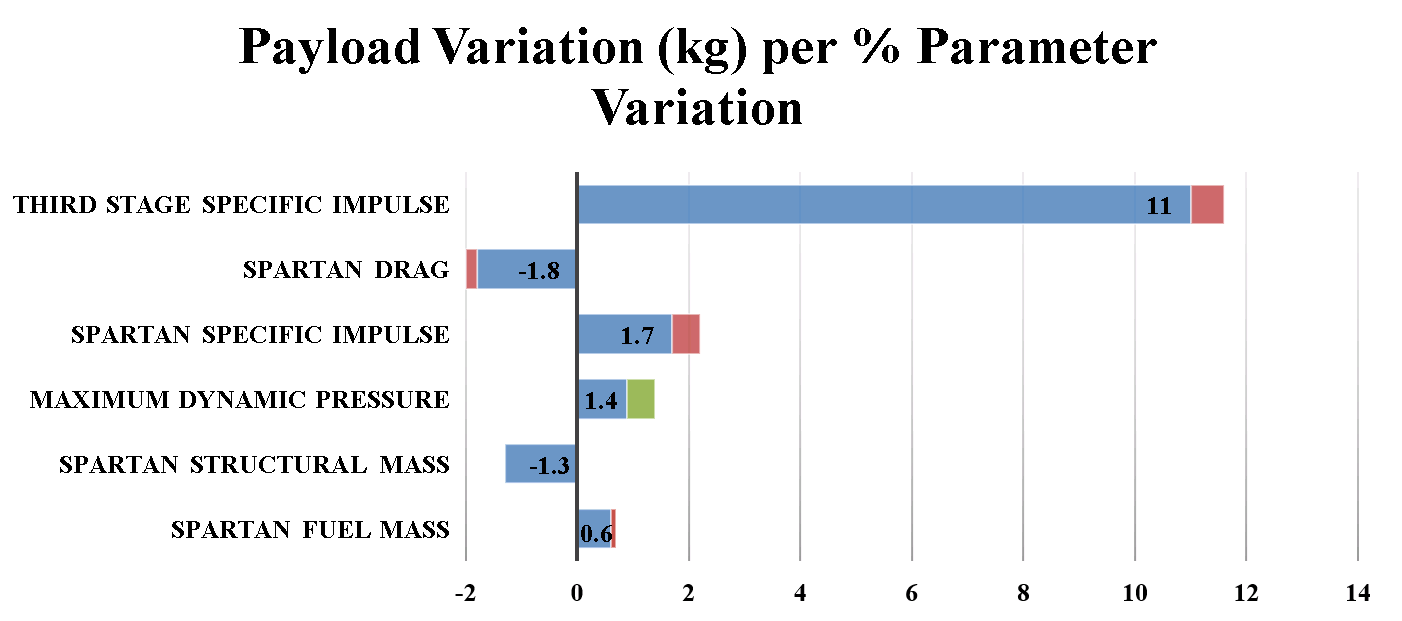
\includegraphics[width=0.99\linewidth]{figures/6_FlyBack/BarChart}
	\caption{The sensitivity of the key design parameters of the launch system, including scramjet accelerator fly-back. Red and green coloured areas indicate decreases or increases in the magnitude of sensitivity respectively, compared to the sensitivity study without scramjet accelerator fly-back in Section \ref{sec:comparisonNoReturn}.}
	\label{fig:BarChartreturn}
\end{figure}

The sensitivities of the performance of the launch system, including the fly-back of the scramjet accelerator, to a variety of design parameters have been presented in the preceding sections. Figure \ref{fig:BarChartreturn} shows a relative comparison of the payload-to-orbit sensitivity for each design parameter, by percentage. The magnitude of each sensitivity is also compared with the sensitivity of the launch system performance without fly-back, detailed in Section \ref{sec:comparisonNoReturn}.

The sensitivity of the launch system to the \textcolor{red}{structural mass of the scramjet accelerator} is unchanged when fly-back is included. However, the increaase in the sensitivity of the launch system to the \textcolor{red}{maximum allowable dynamic pressure}, to \textcolor{red}{1.4}$\frac{\Delta kg}{\Delta\%q_{max}}$, means that the potential beneficial effects of reducing the maximum dynamic pressure of the scramjet accelerator are increased. So long as the mass of the scramjet accelerator \textcolor{red}{is increased} by less than \textcolor{red}{114.4}kg for each 1kPa \textcolor{red}{increase} in the maximum dynamic pressure, the performance of the launch system will improve.
 The sensitivity of the launch system to the specific impulse of the scramjet accelerator is decreased significantly when the fly-back of the scramjet accelerator is included, to \textcolor{red}{1.7}$\frac{\Delta kg}{\Delta\%I_{SP,scramjet accelerator}}$, a decrease of \textcolor{red}{-0.5}$\frac{\Delta kg}{\Delta\%I_{SP,scramjet accelerator}}$ (\textcolor{red}{-22.7}\%) compared to the sensitivity without fly-back, while the sensitivity of the launch system to the scramjet accelerator's structural mass is unchanged, at \textcolor{red}{-1.3}$\frac{\Delta kg}{\Delta\%m_{scramjet accelerator}}$. Comparing these sensitivities, it is apparent that if the specific impulse of the scramjet accelerator can be increased by 1\% with less than \textcolor{red}{64.8kg} increase in the total mass of the scramjet accelerator, then the overall performance of the launch system will be improved.  
Similarly, the sensitivity of the launch system to variation in the drag of the scramjet accelerator is reduced, to \textcolor{red}{-1.8}$\frac{\Delta kg}{\Delta\%C_{d,scramjet accelerator}}$. Comparing this sensitivity with the sensitivity to the \textcolor{red}{C-REST specific impulse}, the specific impulse of the C-REST engines must be improved by 1\% while increasing the drag of the scramjet accelerator by less than \textcolor{red}{0.9}\% due to shape variation, in order for the overall performance change to be beneficial. 

The \textcolor{red}{unchanged} sensitivity of the launch system performance to the structural mass of the scramjet accelerator, along with the decreased fuel mass sensitivity, means that so long as 1kg of fuel mass can be added with less than \textcolor{red}{1.5}kg of structural mass added, the performance of the launch system will improve. Additionally, the decreased sensitivity of the launch system to the drag of the scramjet accelerator means that so long as 1kg of fuel can be added to the scramjet accelerator, with a drag increase of less than 0.021\% due to increased size, then the maximum payload-to-orbit will increase \textcolor{red}{(assuming lift is unchanged)}. 


\section{Summary}

In this chapter, the maximum payload-to-orbit trajectory for the SPARTAN rocket-scramjet-rocket system has been calculated, with the inclusion of the fly-back of the scramjet accelerator stage. It was found that this launch system is able to deliver \PayloadToOrbitStandard kg of payload to sun synchronous orbit, while successfully returning the scramjet-powered stage to the initial launch site. 
This return flight decreases the payload-to-orbit by -19.0kg (-10\%), but removes the need for the costly and time consuming transportation of the scramjet accelerator after launch, which would be necessary if landing at a downrange location.
During the return flight, the scramjet engines are powered on three times, in total using \returnFuelStandard kg of fuel for the return flight, 17.2\% of the scramjet accelerator's total fuel.

It was found that when the fly-back of the scramjet accelerator is included in the optimal trajectory calculation, the first stage of the launch system pitches in an easterly direction. 
The launch system exhibits a first-second separation point of \firstsecondSeparationAltStandard km, an increase of 3.0km when compared to the maximum payload-to-orbit trajectory with no fly-back, and a trajectory angle of \firstsecondSeparationgammaStandard $^\circ$, an increase of 2.5$^\circ$. 
This higher separation point allows the first stage to efficiently use 17943kg of fuel, as well as increasing its exergy efficiency to \firstExergyEffStandard \%$\eta$, increases of +758kg (+4.4\%) and +0.308\%$\eta$ (+4.9\%) respectively when compared to the maximum payload-to-orbit trajectory with no fly-back.
In addition to increasing the fuel and exergy efficiency of the first stage, the higher first-second separation serves to increase the altitude of the scramjet accelerator at the beginning of its trajectory. This allows the scramjet accelerator time to increase its bank angle, so that when the scramjet accelerator descends it is able to change its heading angle rapidly. The scramjet accelerator maintains a high bank angle throughout its trajectory, executing a banking manoeuvre, and staying close to its maximum dynamic pressure. 
This banking manoeuvre requires higher angles of attack, increasing the drag of the scramjet accelerator, but also reduces the ground distance necessary for the return of the scramjet accelerator, decreasing the amount of fuel necessary for fly-back and increasing the overall efficiency of the scramjet accelerator. 
At the end of its acceleration, the scramjet accelerator was found to exhibit a pull-up manoeuvre before the separation of the third stage, in a similar fashion to the maximum payload-to-orbit trajectory with no fly-back. 

The fly-back of the scramjet accelerator is found to be separated into three stages; an initial turn, a boost phase, and an approach. 
The initial turn takes place immediately after separation, and consists of the scramjet accelerator banking heavily in order to manoeuvre the heading angle back towards the initial launch site. 
During the boost-skip phase the scramjet accelerator exhibits multiple `skipping' manoeuvres. These skipping manoeuvres have been shown in previous literature to extend the flight range of hypersonic vehicles\cite{Moshman2014,Darby2011,Toso2015,Tetlow1992,Eggers1957,Kanda2007,Chai2015}, and serve to reduce the amount of fuel used during the fly-back.
In addition, the skipping manoeuvres allow the scramjet engines to be powered on at the points where the specific impulse of the C-REST engines are highest, maximising the performance of the scramjet accelerator, and minimising the fuel necessary for return. 
During the approach phase, the trajectory of the scramjet accelerator is smoothed, and the scramjet accelerator glides to the landing point. 
 The optimal trajectory terminates when scramjet accelerator reaches 1km altitude at a velocity of 120m/s. After this point, it is assumed that the scramjet accelerator lands on a traditional runway.  
This result indicates that it is feasible to return a hypersonic launch vehicle separated at a high Mach number to its initial launch site, and that a cost efficient mission profile for a rocket-scramjet-rocket launch system is attainable.  

The sensitivity of the launch system to various design parameters has been investigated. 
The payload-to-orbit sensitivity of the launch system to variations in the specific impulse, drag and structural mass of the scramjet accelerator was found to decrease when fly-back is included, compared to the sensitivity study with no fly-back. This decreased sensitivity indicates that the fly-back of the scramjet accelerator offsets some of the payload-to-orbit variation due to changes in these parameters. 
It was found that the first-second separation conditions do not exhibit clear trends with scramjet accelerator performance when fly-back is included, in contrast to the trade-offs observed in Section \ref{sec:sensitivityNoReturn}. The disappearance of these trends indicates that when the fly-back of the scramjet accelerator is included, the first-second separation point is determined by a more complex trade-off. This trade-off involves the banking and manoeuvrability of the scramjet accelerator at the start of its acceleration, which affects the efficiency of the return flight. 
